\section{三角形网格}\label{sec:三角形网格}
\keyindex{三角形}{triangle}{}是计算机图形学最常用的形状;
复杂场景会用上百万三角形建模以实现出色细节
(\reffig{3.11}展示了四百多万三角形的复杂三角网格图像)。
\begin{figure}[htbp]
    \centering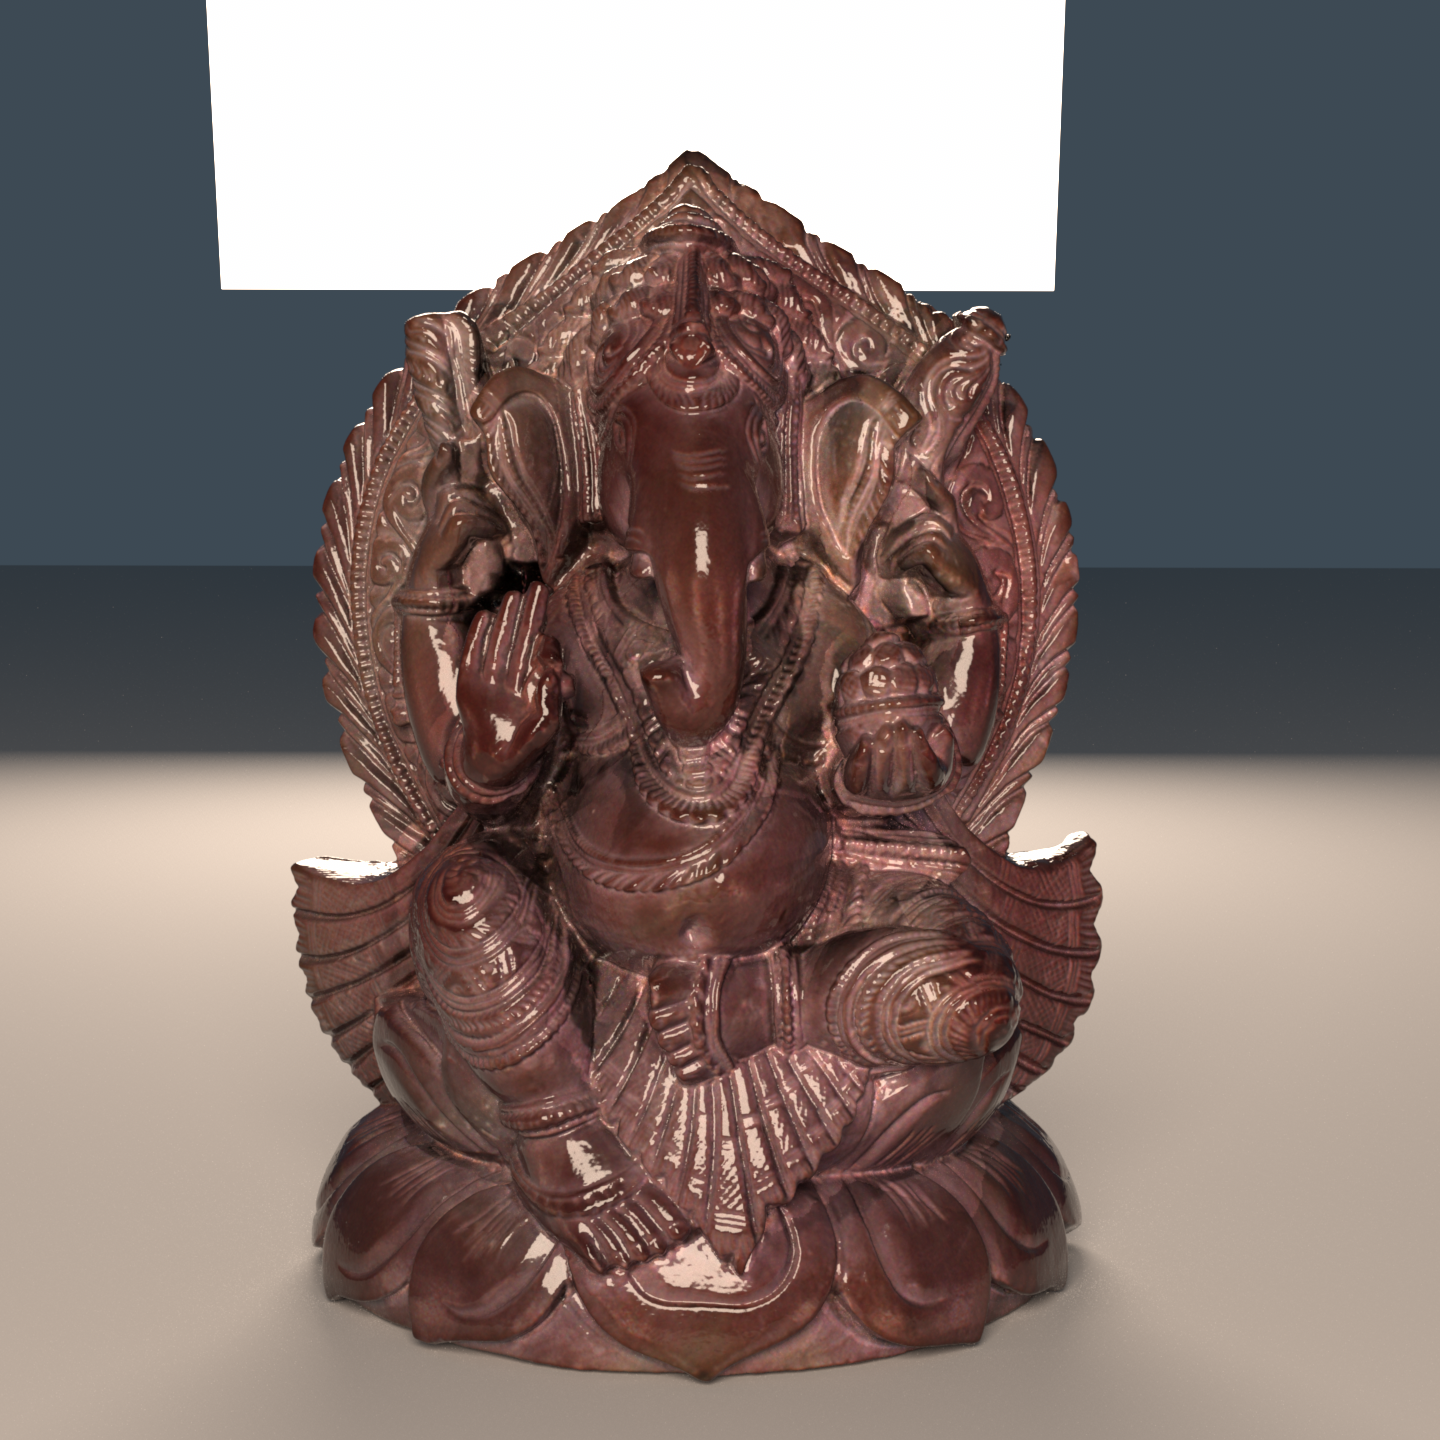
\includegraphics[width=\linewidth]{chap03/ganesha.png}
    \caption{象头神模型。该三角网格含有四百多万个独立三角形。
        它是使用结构光确定物体形状的3D扫描器用真实雕塑创建的。}
    \label{fig:3.11}
\end{figure}

尽管自然的表示是用{\ttfamily Triangle}形状实现,
每个三角形都存储它三个顶点的位置,
但内存更高效的表示是用一个顶点位置数组分开存储整个\keyindex{三角网格}{triangle mesh}{},
每个独立三角形只存储它三个顶点对该数组的三个偏移量。

为了理解为什么是这样,考虑著名的\keyindex{欧拉-庞加莱公式}{Euler-Poincaré formula}{},
它将闭合离散网格的顶点数$V$、边数$E$和面数$F$联系起来:
\begin{align*}
    V-E+F=2(1-g)\, ,
\end{align*}
其中$g\in\mathbb{N}$是网格的\keyindex{亏格}{genus}{}。
亏格通常是很小的数且能解释为网格的“手柄”数量(类似于茶杯把手)。
在三角网格上,边数和面数\sidenote{译者注:原文错写为顶点数,已修改。}还由恒等式联系
\begin{align*}
    E=\frac{3}{2}F\, .
\end{align*}
这可以看作把每条边分成两部分与两个相邻三角形关联。
有$3F$条这样的半边,所有同位的边对构成$E$条网格边。
对于巨大的闭合三角网格,亏格的整体影响通常可以忽略,
我们可以结合之前两个方程(以及$g=0$)得到
\begin{align*}
    F\approx2V\, .
\end{align*}
换句话说,面数大约是顶点数的两倍。
既然每个面引用三个顶点,每个顶点(平均)总共被引用六次。
因此当共享顶点时,每个三角形所需的总分摊存储为
偏移量的12字节内存(三个4字节32位整数偏移量)加上一个顶点存储的一半——6字节,
这里假设每个顶点用三个4字节浮点存储——每个三角形一共18字节。
这比每个三角形直接用36字节存储三个位置好得多。
当网格中有每个顶点的曲面法线或纹理坐标时,相对的存储节约会更好。

pbrt使用结构体\refvar{TriangleMesh}{}保存关于三角网格的共享信息。
\begin{lstlisting}
`\initcode{Triangle Declarations}{=}\initnext{TriangleDeclarations}`
struct `\initvar{TriangleMesh}{}` {
    `\refcode{TriangleMesh Public Methods}{}`
    `\refcode{TriangleMesh Data}{}`
};
\end{lstlisting}
\begin{lstlisting}
`\initcode{TriangleMesh Public Methods}{=}`
`\refvar{TriangleMesh}{}`(const `\refvar{Transform}{}` &ObjectToWorld, int nTriangles, const int *vertexIndices,
    int nVertices, const `\refvar{Point3f}{}` *P, const `\refvar{Vector3f}{}` *S, const `\refvar{Normal3f}{}` *N,
    const `\refvar{Point2f}{}` *uv, const std::shared_ptr<`\refvar{Texture}{}`<`\refvar{Float}{}`>> &alphaMask);
\end{lstlisting}

\refvar{TriangleMesh}{}构造函数的参数如下:
\begin{itemize}
    \item {\ttfamily ObjectToWorld}:网格的物体到世界的变换。
    \item {\ttfamily nTriangles}:网格中三角形总数。
    \item {\ttfamily vertexIndices}:指向顶点索引数组的指针。对于第{\ttfamily i}个三角形,其三个顶点位置为
          {\ttfamily P[vertexIndices[3*i]]}、{\ttfamily P[vertexIndices[3*i+1]]}和{\ttfamily P[vertexIndices[3*i+2]]}。
    \item {\ttfamily nVertices}:网格中顶点总数。
    \item {\ttfamily P}:{\ttfamily nVertices}个顶点位置的数组。
    \item {\ttfamily S}:可选切向量数组,网格中每个顶点都有一个。它们用于计算着色切线。
    \item {\ttfamily N}:可选法向量数组,网格中每个顶点都有一个。如果有,则它们在三角形面之间插值以计算着色法线。
    \item {\ttfamily UV}:可选参数值$(u,v)$数组,每个顶点一个。
    \item {\ttfamily alphaMask}:可选的\keyindex{$\alpha$掩模}{alpha mask}{}纹理,可用于截去部分三角形面。
\end{itemize}

pbrt中三角形在形状里有双重角色:不仅场景描述文件经常直接指定它们,
其他形状也常把自己细分为三角网格。
例如,细分曲面最终创建一个三角网格来近似光滑有限曲面。
再对这些三角形执行光线相交,而不是直接对细分曲面这样做(\refsub{细分})。

由于这第二种角色,创建三角网格的代码能指定三角形的参数化很重要。
如果三角形是通过求取参数化曲面在三个特定坐标值$(u,v)$处的位置来创建的,
这些$(u,v)$值应该被插值以计算三角形内光线交点处的$(u,v)$值。
显式指定$(u,v)$值对纹理贴图也很有用,创建三角网格的外部程序
可能想给网格赋值$(u,v)$坐标,这样纹理贴图以期望的方式把颜色赋值给网格曲面。

\refvar{TriangleMesh}{}构造函数赋值相关信息并存于成员变量中。
特别地,它自己复制{\ttfamily vertexIndices、P、N、S}和{\ttfamily UV},
允许调用者保留对传入数据的所有权。
\begin{lstlisting}
`\initcode{Triangle Method Definitions}{=}\initnext{TriangleMethodDefinitions}`
`\refvar{TriangleMesh}{}`::`\refvar{TriangleMesh}{}`(const `\refvar{Transform}{}` &ObjectToWorld,
        int nTriangles, const int *vertexIndices, int nVertices,
        const `\refvar{Point3f}{}` *P, const `\refvar{Vector3f}{}` *S, const `\refvar{Normal3f}{}` *N,
        const `\refvar{Point3f}{}` *UV,
        const std::shared_ptr<`\refvar{Texture}{}`<`\refvar{Float}{}`>> &alphaMask)
    : `\refvar{nTriangles}{}`(nTriangles), `\refvar{nVertices}{}`(nVertices), 
      `\refvar{vertexIndices}{}`(vertexIndices, vertexIndices + 3 * nTriangles),
      `\refvar{alphaMask}{}`(alphaMask) {
    `\refcode{Transform mesh vertices to world space}{}`
    `\refcode{Copy UV, N, and S vertex data, if present}{}`
}
\end{lstlisting}
\begin{lstlisting}
    `\initcode{TriangleMesh Data}{=}`
    const int `\initvar{nTriangles}{}`, `\initvar{nVertices}{}`;
    std::vector<int> `\initvar{vertexIndices}{}`;
    std::unique_ptr<`\refvar{Point3f}{}`[]> `\initvar[TriangleMesh::p]{p}{}`;
    std::unique_ptr<`\refvar{Normal3f}{}`[]> `\initvar[TriangleMesh::n]{n}{}`;
    std::unique_ptr<`\refvar{Vector3f}{}`[]> `\initvar[TriangleMesh::s]{s}{}`;
    std::unique_ptr<`\refvar{Point2f}{}`[]> `\initvar[TriangleMesh::uv]{uv}{}`;
    std::shared_ptr<`\refvar{Texture}{}`<`\refvar{Float}{}`>> `\initvar{alphaMask}{}`;
\end{lstlisting}

不像其他形状那样把形状描述留在物体空间内然后
将入射光线从世界空间变换到物体空间,
三角网格将形状变换到世界空间,
因此节约了把入射光线变换到物体空间的工作和
把相交处的几何表示变换出世界空间的工作。
这是个好主意,因为该操作可在启动后执行,
避免渲染中多次变换光线。
尽管也能对二次曲面使用该方法,但会更复杂(见本章末习题7了解更多信息)。
\begin{lstlisting}
    `\initcode{Transform mesh vertices to world space}{=}`
    `\refvar[TriangleMesh::p]{p}{}`.reset(new `\refvar{Point3f}{}`[`\refvar{nVertices}{}`]);
    for (int i = 0; i < `\refvar{nVertices}{}`; ++i)
    `\refvar[TriangleMesh::p]{p}{}`[i] = ObjectToWorld(P[i]);
\end{lstlisting}

代码片\refcode{Copy UV, N, and S vertex data, if present}{}只是
分配合适数量的空间并复制合适的值。
如果有法线和切向量,则也变换到世界空间。
\begin{lstlisting}
`\initcode{Copy UV, N, and S vertex data, if present}{=}`
if (UV) {
    `\refvar[TriangleMesh::uv]{uv}{}`.reset(new `\refvar{Point2f}{}`[`\refvar{nVertices}{}`]);
    memcpy(`\refvar[TriangleMesh::uv]{uv}{}`.get(), UV, `\refvar{nVertices}{}` * sizeof(`\refvar{Point2f}{}`));
}
if (N) {
    `\refvar[TriangleMesh::n]{n}{}`.reset(new `\refvar{Normal3f}{}`[`\refvar{nVertices}{}`]);
    for (int i = 0; i < `\refvar{nVertices}{}`; ++i)
        `\refvar[TriangleMesh::n]{n}{}`[i] = ObjectToWorld(N[i]);
}
if (S) {
    `\refvar[TriangleMesh::s]{s}{}`.reset(new `\refvar{Vector3f}{}`[`\refvar{nVertices}{}`]);
    for (int i = 0; i < `\refvar{nVertices}{}`; ++i)
        `\refvar[TriangleMesh::s]{s}{}`[i] = ObjectToWorld(S[i]);
}
\end{lstlisting}

\subsection{三角形}\label{sub:三角形}
类\refvar{Triangle}{}实际上实现了\refvar{Shape}{}接口。它表示单个三角形。
\begin{lstlisting}
`\refcode{Triangle Declarations}{+=}\lastcode{TriangleDeclarations}`
class `\initvar{Triangle}{}` : public `\refvar{Shape}{}` {
public:
    `\refcode{Triangle Public Methods}{}`
private:
    `\refcode{Triangle Private Methods}{}`
    `\refcode{Triangle Private Data}{}`
};
\end{lstlisting}

\refvar{Triangle}{}不存储太多数据——只有一个指向其来处的父\refvar{TriangleMesh}{}指针
和一个指向网格中其三个顶点索引的指针。
\begin{lstlisting}
`\initcode{Triangle Public Methods}{=}`
`\refvar{Triangle}{}`(const `\refvar{Transform}{}` *ObjectToWorld, const `\refvar{Transform}{}` *WorldToObject,
         bool reverseOrientation,
         const std::shared_ptr<`\refvar{TriangleMesh}{}`> &mesh, int triNumber)
    : `\refvar{Shape}{}`(ObjectToWorld, WorldToObject, reverseOrientation),
      `\refvar{mesh}{}`(mesh) {
    `\refvar[Triangle::v]{v}{}` = &mesh->`\refvar{vertexIndices}{}`[3 * triNumber];
}
\end{lstlisting}

注意该实现存储了指向第一个顶点\emph{索引}的指针,
而非存储三个指向顶点自己的指针。
这以另一级别的间接性为代价减少了每个\refvar{Triangle}{}所需的存储量。
\begin{lstlisting}
`\initcode{Triangle Private Data}{=}`
std::shared_ptr<`\refvar{TriangleMesh}{}`> `\initvar{mesh}{}`;
const int *`\initvar[Triangle::v]{v}{}`;
\end{lstlisting}

因为pbrt中大量的其他形状表示会把自己转化为三角网格,
实用函数
\refvar{CreateTriangleMesh}{()}仔细创建
底层\refvar{TriangleMesh}{}以及网格中每个三角形的\refvar{Triangle}{}。
它返回三角形状的向量。
\begin{lstlisting}
`\refcode{Triangle Method Definitions}{+=}\lastnext{TriangleMethodDefinitions}`
std::vector<std::shared_ptr<`\refvar{Shape}{}`>> `\initvar{CreateTriangleMesh}{}`(
        const `\refvar{Transform}{}` *ObjectToWorld, const `\refvar{Transform}{}` *WorldToObject,
        bool reverseOrientation, int nTriangles,
        const int *vertexIndices, int nVertices, const `\refvar{Point3f}{}` *p,
        const `\refvar{Vector3f}{}` *s, const `\refvar{Normal3f}{}` *n, const `\refvar{Point2f}{}` *uv,
        const std::shared_ptr<`\refvar{Texture}{}`<`\refvar{Float}{}`>> &alphaMask) {
    std::shared_ptr<`\refvar{TriangleMesh}{}`> mesh = std::make_shared<`\refvar{TriangleMesh}{}`>(
        *ObjectToWorld, nTriangles, vertexIndices, nVertices, p, s, n, uv,
        alphaMask);
    std::vector<std::shared_ptr<`\refvar{Shape}{}`>> tris;
    for (int i = 0; i < nTriangles; ++i)
        tris.push_back(std::make_shared<`\refvar{Triangle}{}`>(ObjectToWorld,
            WorldToObject, reverseOrientation, mesh, i));
    return tris;
}
\end{lstlisting}

三角形的物体空间边界很容易通过计算包围其三个顶点的边界框求得。
因为顶点位置\refvar[TriangleMesh::p]{p}{}在构造函数中被变换到世界空间,
这里的实现要在计算其边界前把它们变换回物体空间。
\begin{lstlisting}
`\refcode{Triangle Method Definitions}{+=}\lastnext{TriangleMethodDefinitions}`
`\refvar{Bounds3f}{}` `\refvar{Triangle}{}`::`\initvar[Triangle::ObjectBound]{\refvar{ObjectBound}{}}{}`() const {
    `\refcode{Get triangle vertices in p0, p1, and p2}{}`
    return `\refvar[Union1]{Union}{}`(`\refvar{Bounds3f}{}`((*`\refvar{WorldToObject}{}`)(p0), (*`\refvar{WorldToObject}{}`)(p1)),
                 (*`\refvar{WorldToObject}{}`)(p2));
}
\end{lstlisting}
\begin{lstlisting}
`\initcode{Get triangle vertices in p0, p1, and p2}{=}`
const `\refvar{Point3f}{}` &p0 = `\refvar{mesh}{}`->`\refvar[TriangleMesh::p]{p}{}`[`\refvar[Triangle::v]{v}{}`[0]];
const `\refvar{Point3f}{}` &p1 = `\refvar{mesh}{}`->`\refvar[TriangleMesh::p]{p}{}`[`\refvar[Triangle::v]{v}{}`[1]];
const `\refvar{Point3f}{}` &p2 = `\refvar{mesh}{}`->`\refvar[TriangleMesh::p]{p}{}`[`\refvar[Triangle::v]{v}{}`[2]];
\end{lstlisting}

比起变换其物体空间边界框到世界空间,
\refvar{Triangle}{}形状是能计算更好的世界空间边界的形状之一。
其世界空间边界可以直接从世界空间顶点算得。
\begin{lstlisting}
`\refcode{Triangle Method Definitions}{+=}\lastnext{TriangleMethodDefinitions}`
`\refvar{Bounds3f}{}` `\refvar{Triangle}{}`::`\initvar[Triangle::WorldBound]{\refvar[Shape::WorldBound]{WorldBound}{}}{}`() const {
    `\refcode{Get triangle vertices in p0, p1, and p2}{}`
    return `\refvar[Union1]{Union}{}`(`\refvar{Bounds3f}{}`(p0, p1), p2); 
}
\end{lstlisting}

\subsection{三角形相交}\label{sub:三角形相交}
三角形状方法\refvar[Triangle::Intersect]{Intersect}{()}的结构
遵循之前的相交测试方法:应用几何测试以确定是否相交,
如果有,则计算更多关于相交的信息,并在给定的
\refvar{SurfaceInteraction}{}中返回。
\begin{lstlisting}
`\refcode{Triangle Method Definitions}{+=}\lastnext{TriangleMethodDefinitions}`
bool `\initvar{Triangle::Intersect}{}`(const `\refvar{Ray}{}` &ray, `\refvar{Float}{}` *tHit,
        `\refvar{SurfaceInteraction}{}` *isect, bool testAlphaTexture) const {
    `\refcode{Get triangle vertices in p0, p1, and p2}{}`
    `\refcode{Perform ray–triangle intersection test}{}`
    `\refcode{Compute triangle partial derivatives}{}`
    `\refcode{Compute error bounds for triangle intersection}{}`
    `\refcode{Interpolate (u,v) parametric coordinates and hit point}{}`
    `\refcode{Test intersection against alpha texture, if present}{}`
    `\refcode{Fill in SurfaceInteraction from triangle hit}{}`
    *tHit = t;
    return true;
}
\end{lstlisting}

pbrt的光线-三角形相交测试基于首先计算仿射变换
使得射线在变换后的坐标系统里端点被变换为$(0,0,0)$且其方向沿$+z$轴。
在执行相机测试之前三角形顶点也变换到该坐标系统。
下面我们将看到应用该坐标系统变换会简化相交测试逻辑,
例如任何交点的$x$和$y$坐标必须为零。
之后在\refsub{稳定的三角形相交},我们会看到该变换让
拥有\keyindex{水密的}{watertight}{}光线-三角形相交算法成为可能,
这样刚好命中三角形边缘的棘手光线等的相交就永远不会被错误地报告为未命中了。
\begin{lstlisting}
`\initcode{Perform ray–triangle intersection test}{=}`
`\refcode{Transform triangle vertices to ray coordinate space}{}`
`\refcode{Compute edge function coefficients e0, e1, and e2}{}`
`\refcode{Fall back to double-precision test at triangle edges}{}`
`\refcode{Perform triangle edge and determinant tests}{}`
`\refcode{Compute scaled hit distance to triangle and test against ray t range}{}`
`\refcode{Compute barycentric coordinates and t value for triangle intersection}{}`
`\refcode{Ensure that computed triangle t is conservatively greater than zero}{}`
\end{lstlisting}

计算从世界空间到光线-三角形相交坐标空间的变换有三步:
平移$\bm T$、坐标\keyindex{置换}{permutation}{}$\bm P$和\keyindex{错切}{shear}{}$\bm S$。
下列实现没有为它们每个都计算显式的变换矩阵
再计算合成变换矩阵$\bm M=\bm S\bm P\bm T$来把顶点变换到坐标空间,
而是直接施加每步的变换,这最终是更高效的方法。
\begin{lstlisting}
`\initcode{Transform triangle vertices to ray coordinate space}{=}`
`\refcode{Translate vertices based on ray origin}{}`
`\refcode{Permute components of triangle vertices and ray direction}{}`
`\refcode{Apply shear transformation to translated vertex positions}{}`
\end{lstlisting}

将射线端点放置在坐标系统的原点的平移是:
\begin{align*}
    \bm T=\left[\begin{array}{cccc}
            1 & 0 & 0 & -o_x \\
            0 & 1 & 0 & -o_y \\
            0 & 0 & 1 & -o_z \\
            0 & 0 & 0 & 1
        \end{array}\right]\, .
\end{align*}
该变换不需要显式施加到射线端点,但我们会将其施加于三角形三个顶点。
\begin{lstlisting}
`\initcode{Translate vertices based on ray origin}{=}`
`\refvar{Point3f}{}` p0t = p0 - `\refvar{Vector3f}{}`(ray.o);
`\refvar{Point3f}{}` p1t = p1 - `\refvar{Vector3f}{}`(ray.o);
`\refvar{Point3f}{}` p2t = p2 - `\refvar{Vector3f}{}`(ray.o);
\end{lstlisting}

接下来,置换空间三个维度使得$z$维的射线方向绝对值最大。
$x$和$y$维任意分配给另外两维。
例如,这步保证如果原始射线的$z$方向为零,
则非零幅度的维度映射到$+z$。

例如,如果光线方向在$x$有最大幅值,则置换为:
\begin{align*}
    \bm P=\left[\begin{array}{cccc}
            0 & 1 & 0 & 0 \\
            0 & 0 & 1 & 0 \\
            1 & 0 & 0 & 0 \\
            0 & 0 & 0 & 1
        \end{array}\right]\, .
\end{align*}

像之前那样,直接置换射线方向维度和平移后的三角形顶点最简单。
\begin{lstlisting}
`\initcode{Permute components of triangle vertices and ray direction}{=}`
int kz = `\refvar{MaxDimension}{}`(`\refvar[Vector3::Abs]{Abs}{}`(ray.d));
int kx = kz + 1; if (kx == 3) kx = 0;
int ky = kx + 1; if (ky == 3) ky = 0;
`\refvar{Vector3f}{}` d = `\refvar[Vector3::Permute]{Permute}{}`(ray.d, kx, ky, kz);
p0t = `\refvar[Point3::Permute]{Permute}{}`(p0t, kx, ky, kz);
p1t = `\refvar[Point3::Permute]{Permute}{}`(p1t, kx, ky, kz);
p2t = `\refvar[Point3::Permute]{Permute}{}`(p2t, kx, ky, kz);
\end{lstlisting}

最后,错切变换将射线方向与$+z$轴对齐:
\begin{align*}
    \bm S=\left[\begin{array}{rrrr}
            1 & 0 & \displaystyle-\frac{d_x}{d_z} & 0 \\
            0 & 1 & \displaystyle-\frac{d_y}{d_z} & 0 \\
            0 & 0 & \displaystyle\frac{1}{d_z}    & 0 \\
            0 & 0 & 0                             & 1
        \end{array}\right]\, .
\end{align*}
为了理解该变换如何工作,可考虑它对射线方向向量$[d_x\ d_y\ d_z\ 0]^{\mathrm{T}}$的操作。

现在,只有$x$和$y$维被错切;我们可以等到只有当光线确实与三角形相交时再错切$z$维。
\begin{lstlisting}
`\initcode{Apply shear transformation to translated vertex positions}{=}`
`\refvar{Float}{}` Sx = -d.x / d.z;
`\refvar{Float}{}` Sy = -d.y / d.z;
`\refvar{Float}{}` Sz = 1.f / d.z;
p0t.x += Sx * p0t.z;
p0t.y += Sy * p0t.z;
p1t.x += Sx * p1t.z;
p1t.y += Sy * p1t.z;
p2t.x += Sx * p2t.z;
p2t.y += Sy * p2t.z;
\end{lstlisting}

注意坐标置换和错切系数的计算只取决于给定的光线;
它们和三角形无关。在高性能光线追踪器里,
我们可能想一次性计算这些值并保存在类\refvar{Ray}{}里,
而不是为与光线相交的每个三角形重新计算它们。

三角形顶点变换到该坐标系统后,我们现在的任务是求从原点出发
并沿$+z$的光线是否与变换后的三角形相交。
因为构造坐标系统的方式,该问题等价于2D问题即
确定$x,y$坐标$(0,0)$是否在三角形的$xy$投影内(\reffig{3.12})。
\begin{figure}[htbp]
    \centering%LaTeX with PSTricks extensions
%%Creator: Inkscape 1.0.1 (3bc2e813f5, 2020-09-07)
%%Please note this file requires PSTricks extensions
\psset{xunit=.5pt,yunit=.5pt,runit=.5pt}
\begin{pspicture}(332.77999878,185.77000427)
{
\newrgbcolor{curcolor}{0 0 0}
\pscustom[linewidth=1,linecolor=curcolor]
{
\newpath
\moveto(221.52,1.94000427)
\lineto(329.48,49.12000427)
\lineto(270.78,181.22000427)
\closepath
}
}
{
\newrgbcolor{curcolor}{0 0 0}
\pscustom[linewidth=1,linecolor=curcolor,linestyle=dashed,dash=4]
{
\newpath
\moveto(94.86000061,84.16000366)
\lineto(281.83999634,84.16000366)
}
}
{
\newrgbcolor{curcolor}{0 0 0}
\pscustom[linewidth=1,linecolor=curcolor]
{
\newpath
\moveto(25.56999969,84.16000366)
\lineto(86.76000214,84.16000366)
}
}
{
\newrgbcolor{curcolor}{0 0 0}
\pscustom[linestyle=none,fillstyle=solid,fillcolor=curcolor]
{
\newpath
\moveto(81.85,78.66000427)
\lineto(86.11,84.16000427)
\lineto(81.85,89.67000427)
\lineto(94.86,84.16000427)
\closepath
}
}
{
\newrgbcolor{curcolor}{0.65098041 0.65098041 0.65098041}
\pscustom[linestyle=none,fillstyle=solid,fillcolor=curcolor]
{
\newpath
\moveto(83.41,79.86000427)
\lineto(93.55,84.16000427)
\lineto(86.74,84.16000427)
\closepath
}
}
{
\newrgbcolor{curcolor}{0.40000001 0.40000001 0.40000001}
\pscustom[linestyle=none,fillstyle=solid,fillcolor=curcolor]
{
\newpath
\moveto(83.41,88.46000427)
\lineto(93.55,84.16000427)
\lineto(86.74,84.16000427)
\closepath
}
}
{
\newrgbcolor{curcolor}{0 0 0}
\pscustom[linestyle=none,fillstyle=solid,fillcolor=curcolor]
{
\newpath
\moveto(28.17999983,84.19000244)
\curveto(28.17999983,86.28377436)(25.64872433,87.33195976)(24.16838347,85.8516189)
\curveto(22.68804261,84.37127804)(23.736228,81.84000254)(25.82999992,81.84000254)
\curveto(27.92377185,81.84000254)(28.97195724,84.37127804)(27.49161638,85.8516189)
\curveto(26.01127552,87.33195976)(23.48000002,86.28377436)(23.48000002,84.19000244)
\curveto(23.48000002,82.09623052)(26.01127552,81.04804512)(27.49161638,82.52838599)
\curveto(28.97195724,84.00872685)(27.92377185,86.54000235)(25.82999992,86.54000235)
\curveto(23.736228,86.54000235)(22.68804261,84.00872685)(24.16838347,82.52838599)
\curveto(25.64872433,81.04804512)(28.17999983,82.09623052)(28.17999983,84.19000244)
\closepath
}
}
{
\newrgbcolor{curcolor}{0 0 0}
\pscustom[linewidth=1,linecolor=curcolor]
{
\newpath
\moveto(28.17999983,84.19000244)
\curveto(28.17999983,86.28377436)(25.64872433,87.33195976)(24.16838347,85.8516189)
\curveto(22.68804261,84.37127804)(23.736228,81.84000254)(25.82999992,81.84000254)
\curveto(27.92377185,81.84000254)(28.97195724,84.37127804)(27.49161638,85.8516189)
\curveto(26.01127552,87.33195976)(23.48000002,86.28377436)(23.48000002,84.19000244)
\curveto(23.48000002,82.09623052)(26.01127552,81.04804512)(27.49161638,82.52838599)
\curveto(28.97195724,84.00872685)(27.92377185,86.54000235)(25.82999992,86.54000235)
\curveto(23.736228,86.54000235)(22.68804261,84.00872685)(24.16838347,82.52838599)
\curveto(25.64872433,81.04804512)(28.17999983,82.09623052)(28.17999983,84.19000244)
\closepath
}
}
{
\newrgbcolor{curcolor}{0 0 0}
\pscustom[linestyle=none,fillstyle=solid,fillcolor=curcolor]
{
\newpath
\moveto(273.01000357,182.92000437)
\curveto(273.01000357,185.01377629)(270.47872807,186.06196169)(268.99838721,184.58162082)
\curveto(267.51804634,183.10127996)(268.56623174,180.57000446)(270.66000366,180.57000446)
\curveto(272.75377558,180.57000446)(273.80196098,183.10127996)(272.32162012,184.58162082)
\curveto(270.84127926,186.06196169)(268.31000376,185.01377629)(268.31000376,182.92000437)
\curveto(268.31000376,180.82623245)(270.84127926,179.77804705)(272.32162012,181.25838791)
\curveto(273.80196098,182.73872877)(272.75377558,185.27000427)(270.66000366,185.27000427)
\curveto(268.56623174,185.27000427)(267.51804634,182.73872877)(268.99838721,181.25838791)
\curveto(270.47872807,179.77804705)(273.01000357,180.82623245)(273.01000357,182.92000437)
\closepath
}
}
{
\newrgbcolor{curcolor}{0 0 0}
\pscustom[linewidth=1,linecolor=curcolor]
{
\newpath
\moveto(273.01000357,182.92000437)
\curveto(273.01000357,185.01377629)(270.47872807,186.06196169)(268.99838721,184.58162082)
\curveto(267.51804634,183.10127996)(268.56623174,180.57000446)(270.66000366,180.57000446)
\curveto(272.75377558,180.57000446)(273.80196098,183.10127996)(272.32162012,184.58162082)
\curveto(270.84127926,186.06196169)(268.31000376,185.01377629)(268.31000376,182.92000437)
\curveto(268.31000376,180.82623245)(270.84127926,179.77804705)(272.32162012,181.25838791)
\curveto(273.80196098,182.73872877)(272.75377558,185.27000427)(270.66000366,185.27000427)
\curveto(268.56623174,185.27000427)(267.51804634,182.73872877)(268.99838721,181.25838791)
\curveto(270.47872807,179.77804705)(273.01000357,180.82623245)(273.01000357,182.92000437)
\closepath
}
}
{
\newrgbcolor{curcolor}{0 0 0}
\pscustom[linestyle=none,fillstyle=solid,fillcolor=curcolor]
{
\newpath
\moveto(223.42000723,2.8500061)
\curveto(223.42000723,4.94377803)(220.88873173,5.99196342)(219.40839087,4.51162256)
\curveto(217.92805001,3.0312817)(218.9762354,0.5000062)(221.07000732,0.5000062)
\curveto(223.16377925,0.5000062)(224.21196464,3.0312817)(222.73162378,4.51162256)
\curveto(221.25128292,5.99196342)(218.72000742,4.94377803)(218.72000742,2.8500061)
\curveto(218.72000742,0.75623418)(221.25128292,-0.29195121)(222.73162378,1.18838965)
\curveto(224.21196464,2.66873051)(223.16377925,5.20000601)(221.07000732,5.20000601)
\curveto(218.9762354,5.20000601)(217.92805001,2.66873051)(219.40839087,1.18838965)
\curveto(220.88873173,-0.29195121)(223.42000723,0.75623418)(223.42000723,2.8500061)
\closepath
}
}
{
\newrgbcolor{curcolor}{0 0 0}
\pscustom[linewidth=1,linecolor=curcolor]
{
\newpath
\moveto(223.42000723,2.8500061)
\curveto(223.42000723,4.94377803)(220.88873173,5.99196342)(219.40839087,4.51162256)
\curveto(217.92805001,3.0312817)(218.9762354,0.5000062)(221.07000732,0.5000062)
\curveto(223.16377925,0.5000062)(224.21196464,3.0312817)(222.73162378,4.51162256)
\curveto(221.25128292,5.99196342)(218.72000742,4.94377803)(218.72000742,2.8500061)
\curveto(218.72000742,0.75623418)(221.25128292,-0.29195121)(222.73162378,1.18838965)
\curveto(224.21196464,2.66873051)(223.16377925,5.20000601)(221.07000732,5.20000601)
\curveto(218.9762354,5.20000601)(217.92805001,2.66873051)(219.40839087,1.18838965)
\curveto(220.88873173,-0.29195121)(223.42000723,0.75623418)(223.42000723,2.8500061)
\closepath
}
}
{
\newrgbcolor{curcolor}{0 0 0}
\pscustom[linestyle=none,fillstyle=solid,fillcolor=curcolor]
{
\newpath
\moveto(332.27999258,50.02000427)
\curveto(332.27999258,52.1137762)(329.74871708,53.16196159)(328.26837622,51.68162073)
\curveto(326.78803536,50.20127987)(327.83622075,47.67000437)(329.92999268,47.67000437)
\curveto(332.0237646,47.67000437)(333.07194999,50.20127987)(331.59160913,51.68162073)
\curveto(330.11126827,53.16196159)(327.57999277,52.1137762)(327.57999277,50.02000427)
\curveto(327.57999277,47.92623235)(330.11126827,46.87804695)(331.59160913,48.35838782)
\curveto(333.07194999,49.83872868)(332.0237646,52.37000418)(329.92999268,52.37000418)
\curveto(327.83622075,52.37000418)(326.78803536,49.83872868)(328.26837622,48.35838782)
\curveto(329.74871708,46.87804695)(332.27999258,47.92623235)(332.27999258,50.02000427)
\closepath
}
}
{
\newrgbcolor{curcolor}{0 0 0}
\pscustom[linewidth=1,linecolor=curcolor]
{
\newpath
\moveto(332.27999258,50.02000427)
\curveto(332.27999258,52.1137762)(329.74871708,53.16196159)(328.26837622,51.68162073)
\curveto(326.78803536,50.20127987)(327.83622075,47.67000437)(329.92999268,47.67000437)
\curveto(332.0237646,47.67000437)(333.07194999,50.20127987)(331.59160913,51.68162073)
\curveto(330.11126827,53.16196159)(327.57999277,52.1137762)(327.57999277,50.02000427)
\curveto(327.57999277,47.92623235)(330.11126827,46.87804695)(331.59160913,48.35838782)
\curveto(333.07194999,49.83872868)(332.0237646,52.37000418)(329.92999268,52.37000418)
\curveto(327.83622075,52.37000418)(326.78803536,49.83872868)(328.26837622,48.35838782)
\curveto(329.74871708,46.87804695)(332.27999258,47.92623235)(332.27999258,50.02000427)
\closepath
}
}
{
\newrgbcolor{curcolor}{0 0 0}
\pscustom[linewidth=1,linecolor=curcolor]
{
\newpath
\moveto(286.52001333,84.3500061)
\curveto(286.52001333,86.44377803)(283.98873783,87.49196342)(282.50839697,86.01162256)
\curveto(281.02805611,84.5312817)(282.07624151,82.0000062)(284.17001343,82.0000062)
\curveto(286.26378535,82.0000062)(287.31197075,84.5312817)(285.83162988,86.01162256)
\curveto(284.35128902,87.49196342)(281.82001352,86.44377803)(281.82001352,84.3500061)
\curveto(281.82001352,82.25623418)(284.35128902,81.20804879)(285.83162988,82.68838965)
\curveto(287.31197075,84.16873051)(286.26378535,86.70000601)(284.17001343,86.70000601)
\curveto(282.07624151,86.70000601)(281.02805611,84.16873051)(282.50839697,82.68838965)
\curveto(283.98873783,81.20804879)(286.52001333,82.25623418)(286.52001333,84.3500061)
\closepath
}
}
{
\newrgbcolor{curcolor}{0 0 0}
\pscustom[linestyle=none,fillstyle=solid,fillcolor=curcolor]
{
\newpath
\moveto(263.16115708,61.93985942)
\curveto(263.16115708,61.98673442)(263.16115708,62.01017192)(262.90334458,62.26798442)
\curveto(261.05178208,64.14298442)(260.55959458,66.97892192)(260.55959458,69.27579692)
\curveto(260.55959458,71.87735942)(261.12209458,74.47892192)(262.97365708,76.33048442)
\curveto(263.16115708,76.51798442)(263.16115708,76.54142192)(263.16115708,76.58829692)
\curveto(263.16115708,76.70548442)(263.11428208,76.75235942)(263.02053208,76.75235942)
\curveto(262.85646958,76.75235942)(261.52053208,75.72110942)(260.62990708,73.82267192)
\curveto(259.87990708,72.18204692)(259.69240708,70.51798442)(259.69240708,69.27579692)
\curveto(259.69240708,68.10392192)(259.85646958,66.29923442)(260.67678208,64.58829692)
\curveto(261.59084458,62.76017192)(262.85646958,61.77579692)(263.02053208,61.77579692)
\curveto(263.11428208,61.77579692)(263.16115708,61.82267192)(263.16115708,61.93985942)
\closepath
\moveto(263.16115708,61.93985942)
}
}
{
\newrgbcolor{curcolor}{0 0 0}
\pscustom[linestyle=none,fillstyle=solid,fillcolor=curcolor]
{
\newpath
\moveto(270.8947081,70.30704692)
\curveto(270.8947081,71.50235942)(270.8243956,72.69767192)(270.3087706,73.79923442)
\curveto(269.6290831,75.25235942)(268.3868956,75.48673442)(267.7775206,75.48673442)
\curveto(266.8634581,75.48673442)(265.7853331,75.08829692)(265.1525206,73.70548442)
\curveto(264.6837706,72.67423442)(264.6134581,71.50235942)(264.6134581,70.30704692)
\curveto(264.6134581,69.18204692)(264.6603331,67.84610942)(265.2931456,66.69767192)
\curveto(265.9259581,65.50235942)(267.0275206,65.19767192)(267.7540831,65.19767192)
\curveto(268.5509581,65.19767192)(269.6993956,65.50235942)(270.3556456,66.93204692)
\curveto(270.8243956,67.96329692)(270.8947081,69.13517192)(270.8947081,70.30704692)
\closepath
\moveto(267.7540831,65.52579692)
\curveto(267.1681456,65.52579692)(266.2775206,65.90079692)(266.0197081,67.33048442)
\curveto(265.8556456,68.22110942)(265.8556456,69.60392192)(265.8556456,70.49454692)
\curveto(265.8556456,71.45548442)(265.8556456,72.43985942)(265.9728331,73.23673442)
\curveto(266.2540831,75.01798442)(267.3790831,75.15860942)(267.7540831,75.15860942)
\curveto(268.2462706,75.15860942)(269.2306456,74.87735942)(269.5118956,73.40079692)
\curveto(269.6759581,72.55704692)(269.6759581,71.43204692)(269.6759581,70.49454692)
\curveto(269.6759581,69.36954692)(269.6759581,68.36173442)(269.5118956,67.40079692)
\curveto(269.2775206,65.97110942)(268.4337706,65.52579692)(267.7540831,65.52579692)
\closepath
\moveto(267.7540831,65.52579692)
}
}
{
\newrgbcolor{curcolor}{0 0 0}
\pscustom[linestyle=none,fillstyle=solid,fillcolor=curcolor]
{
\newpath
\moveto(274.54671234,65.54923442)
\curveto(274.54671234,66.53360942)(274.17171234,67.11954692)(273.58577484,67.11954692)
\curveto(273.09358734,67.11954692)(272.78889984,66.74454692)(272.78889984,66.32267192)
\curveto(272.78889984,65.92423442)(273.09358734,65.52579692)(273.58577484,65.52579692)
\curveto(273.74983734,65.52579692)(273.96077484,65.59610942)(274.10139984,65.71329692)
\curveto(274.14827484,65.76017192)(274.17171234,65.76017192)(274.17171234,65.76017192)
\curveto(274.19514984,65.76017192)(274.19514984,65.76017192)(274.19514984,65.54923442)
\curveto(274.19514984,64.42423442)(273.67952484,63.53360942)(273.18733734,63.04142192)
\curveto(273.02327484,62.87735942)(273.02327484,62.85392192)(273.02327484,62.80704692)
\curveto(273.02327484,62.68985942)(273.09358734,62.64298442)(273.16389984,62.64298442)
\curveto(273.32796234,62.64298442)(274.54671234,63.79142192)(274.54671234,65.54923442)
\closepath
\moveto(274.54671234,65.54923442)
}
}
{
\newrgbcolor{curcolor}{0 0 0}
\pscustom[linestyle=none,fillstyle=solid,fillcolor=curcolor]
{
\newpath
\moveto(285.00902695,70.30704692)
\curveto(285.00902695,71.50235942)(284.93871445,72.69767192)(284.42308945,73.79923442)
\curveto(283.74340195,75.25235942)(282.50121445,75.48673442)(281.89183945,75.48673442)
\curveto(280.97777695,75.48673442)(279.89965195,75.08829692)(279.26683945,73.70548442)
\curveto(278.79808945,72.67423442)(278.72777695,71.50235942)(278.72777695,70.30704692)
\curveto(278.72777695,69.18204692)(278.77465195,67.84610942)(279.40746445,66.69767192)
\curveto(280.04027695,65.50235942)(281.14183945,65.19767192)(281.86840195,65.19767192)
\curveto(282.66527695,65.19767192)(283.81371445,65.50235942)(284.46996445,66.93204692)
\curveto(284.93871445,67.96329692)(285.00902695,69.13517192)(285.00902695,70.30704692)
\closepath
\moveto(281.86840195,65.52579692)
\curveto(281.28246445,65.52579692)(280.39183945,65.90079692)(280.13402695,67.33048442)
\curveto(279.96996445,68.22110942)(279.96996445,69.60392192)(279.96996445,70.49454692)
\curveto(279.96996445,71.45548442)(279.96996445,72.43985942)(280.08715195,73.23673442)
\curveto(280.36840195,75.01798442)(281.49340195,75.15860942)(281.86840195,75.15860942)
\curveto(282.36058945,75.15860942)(283.34496445,74.87735942)(283.62621445,73.40079692)
\curveto(283.79027695,72.55704692)(283.79027695,71.43204692)(283.79027695,70.49454692)
\curveto(283.79027695,69.36954692)(283.79027695,68.36173442)(283.62621445,67.40079692)
\curveto(283.39183945,65.97110942)(282.54808945,65.52579692)(281.86840195,65.52579692)
\closepath
\moveto(281.86840195,65.52579692)
}
}
{
\newrgbcolor{curcolor}{0 0 0}
\pscustom[linestyle=none,fillstyle=solid,fillcolor=curcolor]
{
\newpath
\moveto(288.66021866,65.54923442)
\curveto(288.66021866,66.53360942)(288.28521866,67.11954692)(287.69928116,67.11954692)
\curveto(287.20709366,67.11954692)(286.90240616,66.74454692)(286.90240616,66.32267192)
\curveto(286.90240616,65.92423442)(287.20709366,65.52579692)(287.69928116,65.52579692)
\curveto(287.86334366,65.52579692)(288.07428116,65.59610942)(288.21490616,65.71329692)
\curveto(288.26178116,65.76017192)(288.28521866,65.76017192)(288.28521866,65.76017192)
\curveto(288.30865616,65.76017192)(288.30865616,65.76017192)(288.30865616,65.54923442)
\curveto(288.30865616,64.42423442)(287.79303116,63.53360942)(287.30084366,63.04142192)
\curveto(287.13678116,62.87735942)(287.13678116,62.85392192)(287.13678116,62.80704692)
\curveto(287.13678116,62.68985942)(287.20709366,62.64298442)(287.27740616,62.64298442)
\curveto(287.44146866,62.64298442)(288.66021866,63.79142192)(288.66021866,65.54923442)
\closepath
\moveto(288.66021866,65.54923442)
}
}
{
\newrgbcolor{curcolor}{0 0 0}
\pscustom[linestyle=none,fillstyle=solid,fillcolor=curcolor]
{
\newpath
\moveto(294.25256867,66.76798442)
\curveto(295.04944367,67.63517192)(295.49475617,68.01017192)(296.03381867,68.47892192)
\curveto(296.03381867,68.47892192)(296.94788117,69.27579692)(297.48694367,69.81485942)
\curveto(298.91663117,71.19767192)(299.24475617,71.92423442)(299.24475617,71.99454692)
\curveto(299.24475617,72.13517192)(299.10413117,72.13517192)(299.08069367,72.13517192)
\curveto(298.96350617,72.13517192)(298.94006867,72.11173442)(298.84631867,71.97110942)
\curveto(298.40100617,71.24454692)(298.09631867,71.01017192)(297.74475617,71.01017192)
\curveto(297.36975617,71.01017192)(297.20569367,71.24454692)(296.97131867,71.50235942)
\curveto(296.69006867,71.83048442)(296.43225617,72.13517192)(295.94006867,72.13517192)
\curveto(294.81506867,72.13517192)(294.13538117,70.75235942)(294.13538117,70.42423442)
\curveto(294.13538117,70.35392192)(294.18225617,70.26017192)(294.29944367,70.26017192)
\curveto(294.44006867,70.26017192)(294.46350617,70.33048442)(294.51038117,70.42423442)
\curveto(294.79163117,71.12735942)(295.65881867,71.12735942)(295.77600617,71.12735942)
\curveto(296.08069367,71.12735942)(296.36194367,71.03360942)(296.71350617,70.91642192)
\curveto(297.32288117,70.68204692)(297.48694367,70.68204692)(297.86194367,70.68204692)
\curveto(297.32288117,70.04923442)(296.08069367,68.97110942)(295.79944367,68.73673442)
\lineto(294.44006867,67.47110942)
\curveto(293.43225617,66.46329692)(292.89319367,65.61954692)(292.89319367,65.50235942)
\curveto(292.89319367,65.36173442)(293.05725617,65.36173442)(293.08069367,65.36173442)
\curveto(293.19788117,65.36173442)(293.22131867,65.38517192)(293.31506867,65.54923442)
\curveto(293.66663117,66.08829692)(294.11194367,66.48673442)(294.60413117,66.48673442)
\curveto(294.93225617,66.48673442)(295.09631867,66.34610942)(295.47131867,65.92423442)
\curveto(295.70569367,65.59610942)(295.98694367,65.36173442)(296.40881867,65.36173442)
\curveto(297.90881867,65.36173442)(298.77600617,67.26017192)(298.77600617,67.65860942)
\curveto(298.77600617,67.72892192)(298.70569367,67.82267192)(298.58850617,67.82267192)
\curveto(298.44788117,67.82267192)(298.42444367,67.72892192)(298.37756867,67.61173442)
\curveto(298.02600617,66.65079692)(297.06506867,66.36954692)(296.57288117,66.36954692)
\curveto(296.29163117,66.36954692)(296.01038117,66.46329692)(295.70569367,66.55704692)
\curveto(295.19006867,66.74454692)(294.95569367,66.81485942)(294.65100617,66.81485942)
\curveto(294.62756867,66.81485942)(294.39319367,66.81485942)(294.25256867,66.76798442)
\closepath
\moveto(294.25256867,66.76798442)
}
}
{
\newrgbcolor{curcolor}{0 0 0}
\pscustom[linestyle=none,fillstyle=solid,fillcolor=curcolor]
{
\newpath
\moveto(302.88528199,76.64210704)
\curveto(302.97903199,76.80616954)(302.97903199,76.89991954)(302.97903199,76.97023204)
\curveto(302.97903199,77.29835704)(302.69778199,77.53273204)(302.36965699,77.53273204)
\curveto(301.97121949,77.53273204)(301.85403199,77.20460704)(301.80715699,77.04054454)
\lineto(300.42434449,72.51710704)
\curveto(300.40090699,72.49366954)(300.35403199,72.37648204)(300.35403199,72.35304454)
\curveto(300.35403199,72.23585704)(300.68215699,72.11866954)(300.77590699,72.11866954)
\curveto(300.84621949,72.11866954)(300.84621949,72.14210704)(300.91653199,72.30616954)
\closepath
\moveto(302.88528199,76.64210704)
}
}
{
\newrgbcolor{curcolor}{0 0 0}
\pscustom[linestyle=none,fillstyle=solid,fillcolor=curcolor]
{
\newpath
\moveto(308.36684174,69.27579692)
\curveto(308.36684174,70.42423442)(308.20277924,72.22892192)(307.38246674,73.93985942)
\curveto(306.49184174,75.76798442)(305.20277924,76.75235942)(305.06215424,76.75235942)
\curveto(304.96840424,76.75235942)(304.89809174,76.68204692)(304.89809174,76.58829692)
\curveto(304.89809174,76.54142192)(304.89809174,76.51798442)(305.17934174,76.23673442)
\curveto(306.65590424,74.76017192)(307.49965424,72.39298442)(307.49965424,69.27579692)
\curveto(307.49965424,66.69767192)(306.96059174,64.07267192)(305.10902924,62.19767192)
\curveto(304.89809174,62.01017192)(304.89809174,61.98673442)(304.89809174,61.93985942)
\curveto(304.89809174,61.84610942)(304.96840424,61.77579692)(305.06215424,61.77579692)
\curveto(305.20277924,61.77579692)(306.56215424,62.80704692)(307.42934174,64.70548442)
\curveto(308.20277924,66.34610942)(308.36684174,68.01017192)(308.36684174,69.27579692)
\closepath
\moveto(308.36684174,69.27579692)
}
}
{
\newrgbcolor{curcolor}{0 0 0}
\pscustom[linestyle=none,fillstyle=solid,fillcolor=curcolor]
{
\newpath
\moveto(9.53065708,62.57156672)
\curveto(9.53065708,62.61844172)(9.53065708,62.64187922)(9.27284458,62.89969172)
\curveto(7.42128208,64.77469172)(6.92909458,67.61062922)(6.92909458,69.90750422)
\curveto(6.92909458,72.50906672)(7.49159458,75.11062922)(9.34315708,76.96219172)
\curveto(9.53065708,77.14969172)(9.53065708,77.17312922)(9.53065708,77.22000422)
\curveto(9.53065708,77.33719172)(9.48378208,77.38406672)(9.39003208,77.38406672)
\curveto(9.22596958,77.38406672)(7.89003208,76.35281672)(6.99940708,74.45437922)
\curveto(6.24940708,72.81375422)(6.06190708,71.14969172)(6.06190708,69.90750422)
\curveto(6.06190708,68.73562922)(6.22596958,66.93094172)(7.04628208,65.22000422)
\curveto(7.96034458,63.39187922)(9.22596958,62.40750422)(9.39003208,62.40750422)
\curveto(9.48378208,62.40750422)(9.53065708,62.45437922)(9.53065708,62.57156672)
\closepath
\moveto(9.53065708,62.57156672)
}
}
{
\newrgbcolor{curcolor}{0 0 0}
\pscustom[linestyle=none,fillstyle=solid,fillcolor=curcolor]
{
\newpath
\moveto(17.2642081,70.93875422)
\curveto(17.2642081,72.13406672)(17.1938956,73.32937922)(16.6782706,74.43094172)
\curveto(15.9985831,75.88406672)(14.7563956,76.11844172)(14.1470206,76.11844172)
\curveto(13.2329581,76.11844172)(12.1548331,75.72000422)(11.5220206,74.33719172)
\curveto(11.0532706,73.30594172)(10.9829581,72.13406672)(10.9829581,70.93875422)
\curveto(10.9829581,69.81375422)(11.0298331,68.47781672)(11.6626456,67.32937922)
\curveto(12.2954581,66.13406672)(13.3970206,65.82937922)(14.1235831,65.82937922)
\curveto(14.9204581,65.82937922)(16.0688956,66.13406672)(16.7251456,67.56375422)
\curveto(17.1938956,68.59500422)(17.2642081,69.76687922)(17.2642081,70.93875422)
\closepath
\moveto(14.1235831,66.15750422)
\curveto(13.5376456,66.15750422)(12.6470206,66.53250422)(12.3892081,67.96219172)
\curveto(12.2251456,68.85281672)(12.2251456,70.23562922)(12.2251456,71.12625422)
\curveto(12.2251456,72.08719172)(12.2251456,73.07156672)(12.3423331,73.86844172)
\curveto(12.6235831,75.64969172)(13.7485831,75.79031672)(14.1235831,75.79031672)
\curveto(14.6157706,75.79031672)(15.6001456,75.50906672)(15.8813956,74.03250422)
\curveto(16.0454581,73.18875422)(16.0454581,72.06375422)(16.0454581,71.12625422)
\curveto(16.0454581,70.00125422)(16.0454581,68.99344172)(15.8813956,68.03250422)
\curveto(15.6470206,66.60281672)(14.8032706,66.15750422)(14.1235831,66.15750422)
\closepath
\moveto(14.1235831,66.15750422)
}
}
{
\newrgbcolor{curcolor}{0 0 0}
\pscustom[linestyle=none,fillstyle=solid,fillcolor=curcolor]
{
\newpath
\moveto(20.91621234,66.18094172)
\curveto(20.91621234,67.16531672)(20.54121234,67.75125422)(19.95527484,67.75125422)
\curveto(19.46308734,67.75125422)(19.15839984,67.37625422)(19.15839984,66.95437922)
\curveto(19.15839984,66.55594172)(19.46308734,66.15750422)(19.95527484,66.15750422)
\curveto(20.11933734,66.15750422)(20.33027484,66.22781672)(20.47089984,66.34500422)
\curveto(20.51777484,66.39187922)(20.54121234,66.39187922)(20.54121234,66.39187922)
\curveto(20.56464984,66.39187922)(20.56464984,66.39187922)(20.56464984,66.18094172)
\curveto(20.56464984,65.05594172)(20.04902484,64.16531672)(19.55683734,63.67312922)
\curveto(19.39277484,63.50906672)(19.39277484,63.48562922)(19.39277484,63.43875422)
\curveto(19.39277484,63.32156672)(19.46308734,63.27469172)(19.53339984,63.27469172)
\curveto(19.69746234,63.27469172)(20.91621234,64.42312922)(20.91621234,66.18094172)
\closepath
\moveto(20.91621234,66.18094172)
}
}
{
\newrgbcolor{curcolor}{0 0 0}
\pscustom[linestyle=none,fillstyle=solid,fillcolor=curcolor]
{
\newpath
\moveto(31.37852695,70.93875422)
\curveto(31.37852695,72.13406672)(31.30821445,73.32937922)(30.79258945,74.43094172)
\curveto(30.11290195,75.88406672)(28.87071445,76.11844172)(28.26133945,76.11844172)
\curveto(27.34727695,76.11844172)(26.26915195,75.72000422)(25.63633945,74.33719172)
\curveto(25.16758945,73.30594172)(25.09727695,72.13406672)(25.09727695,70.93875422)
\curveto(25.09727695,69.81375422)(25.14415195,68.47781672)(25.77696445,67.32937922)
\curveto(26.40977695,66.13406672)(27.51133945,65.82937922)(28.23790195,65.82937922)
\curveto(29.03477695,65.82937922)(30.18321445,66.13406672)(30.83946445,67.56375422)
\curveto(31.30821445,68.59500422)(31.37852695,69.76687922)(31.37852695,70.93875422)
\closepath
\moveto(28.23790195,66.15750422)
\curveto(27.65196445,66.15750422)(26.76133945,66.53250422)(26.50352695,67.96219172)
\curveto(26.33946445,68.85281672)(26.33946445,70.23562922)(26.33946445,71.12625422)
\curveto(26.33946445,72.08719172)(26.33946445,73.07156672)(26.45665195,73.86844172)
\curveto(26.73790195,75.64969172)(27.86290195,75.79031672)(28.23790195,75.79031672)
\curveto(28.73008945,75.79031672)(29.71446445,75.50906672)(29.99571445,74.03250422)
\curveto(30.15977695,73.18875422)(30.15977695,72.06375422)(30.15977695,71.12625422)
\curveto(30.15977695,70.00125422)(30.15977695,68.99344172)(29.99571445,68.03250422)
\curveto(29.76133945,66.60281672)(28.91758945,66.15750422)(28.23790195,66.15750422)
\closepath
\moveto(28.23790195,66.15750422)
}
}
{
\newrgbcolor{curcolor}{0 0 0}
\pscustom[linestyle=none,fillstyle=solid,fillcolor=curcolor]
{
\newpath
\moveto(35.02971866,66.18094172)
\curveto(35.02971866,67.16531672)(34.65471866,67.75125422)(34.06878116,67.75125422)
\curveto(33.57659366,67.75125422)(33.27190616,67.37625422)(33.27190616,66.95437922)
\curveto(33.27190616,66.55594172)(33.57659366,66.15750422)(34.06878116,66.15750422)
\curveto(34.23284366,66.15750422)(34.44378116,66.22781672)(34.58440616,66.34500422)
\curveto(34.63128116,66.39187922)(34.65471866,66.39187922)(34.65471866,66.39187922)
\curveto(34.67815616,66.39187922)(34.67815616,66.39187922)(34.67815616,66.18094172)
\curveto(34.67815616,65.05594172)(34.16253116,64.16531672)(33.67034366,63.67312922)
\curveto(33.50628116,63.50906672)(33.50628116,63.48562922)(33.50628116,63.43875422)
\curveto(33.50628116,63.32156672)(33.57659366,63.27469172)(33.64690616,63.27469172)
\curveto(33.81096866,63.27469172)(35.02971866,64.42312922)(35.02971866,66.18094172)
\closepath
\moveto(35.02971866,66.18094172)
}
}
{
\newrgbcolor{curcolor}{0 0 0}
\pscustom[linestyle=none,fillstyle=solid,fillcolor=curcolor]
{
\newpath
\moveto(45.49202182,70.93875422)
\curveto(45.49202182,72.13406672)(45.42170932,73.32937922)(44.90608432,74.43094172)
\curveto(44.22639682,75.88406672)(42.98420932,76.11844172)(42.37483432,76.11844172)
\curveto(41.46077182,76.11844172)(40.38264682,75.72000422)(39.74983432,74.33719172)
\curveto(39.28108432,73.30594172)(39.21077182,72.13406672)(39.21077182,70.93875422)
\curveto(39.21077182,69.81375422)(39.25764682,68.47781672)(39.89045932,67.32937922)
\curveto(40.52327182,66.13406672)(41.62483432,65.82937922)(42.35139682,65.82937922)
\curveto(43.14827182,65.82937922)(44.29670932,66.13406672)(44.95295932,67.56375422)
\curveto(45.42170932,68.59500422)(45.49202182,69.76687922)(45.49202182,70.93875422)
\closepath
\moveto(42.35139682,66.15750422)
\curveto(41.76545932,66.15750422)(40.87483432,66.53250422)(40.61702182,67.96219172)
\curveto(40.45295932,68.85281672)(40.45295932,70.23562922)(40.45295932,71.12625422)
\curveto(40.45295932,72.08719172)(40.45295932,73.07156672)(40.57014682,73.86844172)
\curveto(40.85139682,75.64969172)(41.97639682,75.79031672)(42.35139682,75.79031672)
\curveto(42.84358432,75.79031672)(43.82795932,75.50906672)(44.10920932,74.03250422)
\curveto(44.27327182,73.18875422)(44.27327182,72.06375422)(44.27327182,71.12625422)
\curveto(44.27327182,70.00125422)(44.27327182,68.99344172)(44.10920932,68.03250422)
\curveto(43.87483432,66.60281672)(43.03108432,66.15750422)(42.35139682,66.15750422)
\closepath
\moveto(42.35139682,66.15750422)
}
}
{
\newrgbcolor{curcolor}{0 0 0}
\pscustom[linestyle=none,fillstyle=solid,fillcolor=curcolor]
{
\newpath
\moveto(50.40928485,69.90750422)
\curveto(50.40928485,71.05594172)(50.24522235,72.86062922)(49.42490985,74.57156672)
\curveto(48.53428485,76.39969172)(47.24522235,77.38406672)(47.10459735,77.38406672)
\curveto(47.01084735,77.38406672)(46.94053485,77.31375422)(46.94053485,77.22000422)
\curveto(46.94053485,77.17312922)(46.94053485,77.14969172)(47.22178485,76.86844172)
\curveto(48.69834735,75.39187922)(49.54209735,73.02469172)(49.54209735,69.90750422)
\curveto(49.54209735,67.32937922)(49.00303485,64.70437922)(47.15147235,62.82937922)
\curveto(46.94053485,62.64187922)(46.94053485,62.61844172)(46.94053485,62.57156672)
\curveto(46.94053485,62.47781672)(47.01084735,62.40750422)(47.10459735,62.40750422)
\curveto(47.24522235,62.40750422)(48.60459735,63.43875422)(49.47178485,65.33719172)
\curveto(50.24522235,66.97781672)(50.40928485,68.64187922)(50.40928485,69.90750422)
\closepath
\moveto(50.40928485,69.90750422)
}
}
{
\newrgbcolor{curcolor}{0 0 0}
\pscustom[linestyle=none,fillstyle=solid,fillcolor=curcolor]
{
\newpath
\moveto(84.61229408,68.02354842)
\lineto(88.78416908,68.02354842)
\curveto(88.99510658,68.02354842)(89.27635658,68.02354842)(89.27635658,68.32823592)
\curveto(89.27635658,68.60948592)(88.99510658,68.60948592)(88.78416908,68.60948592)
\lineto(84.61229408,68.60948592)
\lineto(84.61229408,72.80479842)
\curveto(84.61229408,73.01573592)(84.61229408,73.29698592)(84.30760658,73.29698592)
\curveto(84.00291908,73.29698592)(84.00291908,73.01573592)(84.00291908,72.80479842)
\lineto(84.00291908,68.60948592)
\lineto(79.83104408,68.60948592)
\curveto(79.62010658,68.60948592)(79.33885658,68.60948592)(79.33885658,68.32823592)
\curveto(79.33885658,68.02354842)(79.62010658,68.02354842)(79.83104408,68.02354842)
\lineto(84.00291908,68.02354842)
\lineto(84.00291908,63.82823592)
\curveto(84.00291908,63.61729842)(84.00291908,63.33604842)(84.30760658,63.33604842)
\curveto(84.61229408,63.33604842)(84.61229408,63.61729842)(84.61229408,63.82823592)
\closepath
\moveto(84.61229408,68.02354842)
}
}
{
\newrgbcolor{curcolor}{0 0 0}
\pscustom[linestyle=none,fillstyle=solid,fillcolor=curcolor]
{
\newpath
\moveto(92.1107949,65.82042342)
\curveto(92.9076699,66.68761092)(93.3529824,67.06261092)(93.8920449,67.53136092)
\curveto(93.8920449,67.53136092)(94.8061074,68.32823592)(95.3451699,68.86729842)
\curveto(96.7748574,70.25011092)(97.1029824,70.97667342)(97.1029824,71.04698592)
\curveto(97.1029824,71.18761092)(96.9623574,71.18761092)(96.9389199,71.18761092)
\curveto(96.8217324,71.18761092)(96.7982949,71.16417342)(96.7045449,71.02354842)
\curveto(96.2592324,70.29698592)(95.9545449,70.06261092)(95.6029824,70.06261092)
\curveto(95.2279824,70.06261092)(95.0639199,70.29698592)(94.8295449,70.55479842)
\curveto(94.5482949,70.88292342)(94.2904824,71.18761092)(93.7982949,71.18761092)
\curveto(92.6732949,71.18761092)(91.9936074,69.80479842)(91.9936074,69.47667342)
\curveto(91.9936074,69.40636092)(92.0404824,69.31261092)(92.1576699,69.31261092)
\curveto(92.2982949,69.31261092)(92.3217324,69.38292342)(92.3686074,69.47667342)
\curveto(92.6498574,70.17979842)(93.5170449,70.17979842)(93.6342324,70.17979842)
\curveto(93.9389199,70.17979842)(94.2201699,70.08604842)(94.5717324,69.96886092)
\curveto(95.1811074,69.73448592)(95.3451699,69.73448592)(95.7201699,69.73448592)
\curveto(95.1811074,69.10167342)(93.9389199,68.02354842)(93.6576699,67.78917342)
\lineto(92.2982949,66.52354842)
\curveto(91.2904824,65.51573592)(90.7514199,64.67198592)(90.7514199,64.55479842)
\curveto(90.7514199,64.41417342)(90.9154824,64.41417342)(90.9389199,64.41417342)
\curveto(91.0561074,64.41417342)(91.0795449,64.43761092)(91.1732949,64.60167342)
\curveto(91.5248574,65.14073592)(91.9701699,65.53917342)(92.4623574,65.53917342)
\curveto(92.7904824,65.53917342)(92.9545449,65.39854842)(93.3295449,64.97667342)
\curveto(93.5639199,64.64854842)(93.8451699,64.41417342)(94.2670449,64.41417342)
\curveto(95.7670449,64.41417342)(96.6342324,66.31261092)(96.6342324,66.71104842)
\curveto(96.6342324,66.78136092)(96.5639199,66.87511092)(96.4467324,66.87511092)
\curveto(96.3061074,66.87511092)(96.2826699,66.78136092)(96.2357949,66.66417342)
\curveto(95.8842324,65.70323592)(94.9232949,65.42198592)(94.4311074,65.42198592)
\curveto(94.1498574,65.42198592)(93.8686074,65.51573592)(93.5639199,65.60948592)
\curveto(93.0482949,65.79698592)(92.8139199,65.86729842)(92.5092324,65.86729842)
\curveto(92.4857949,65.86729842)(92.2514199,65.86729842)(92.1107949,65.82042342)
\closepath
\moveto(92.1107949,65.82042342)
}
}
\end{pspicture}

    \caption{在光线-三角形相交坐标系统中,从原点出发的光线沿$+z$轴射出。
        可通过只考虑光线和三角形顶点的$xy$投影执行相交测试,
        转而简化为确定2D点$(0,0)$是否在三角形内。}
    \label{fig:3.12}
\end{figure}

为了理解相交算法如何工作,首先回想\reffig{2.5}中两个向量
叉积的长度给出了它们定义的平行四边形面积。
在2D中,向量为$\bm a$和$\bm b$,则面积为
\begin{align*}
    a_xb_y-b_xa_y\, .
\end{align*}
该面积的一半是它们定义的三角形面积。因此我们看到在2D中,
顶点为$\bm p_0,\bm p_1$和$\bm p_2$的三角形面积为
\begin{align*}
    \frac{1}{2}((p_{1x}-p_{0x})(p_{2y}-p_{0y})-(p_{2x}-p_{0x})(p_{1y}-p_{0y}))\, .
\end{align*}
\reffig{3.13}以几何方式将其可视化。
\begin{figure}[htbp]
    \centering%LaTeX with PSTricks extensions
%%Creator: Inkscape 1.0.1 (3bc2e813f5, 2020-09-07)
%%Please note this file requires PSTricks extensions
\psset{xunit=.5pt,yunit=.5pt,runit=.5pt}
\begin{pspicture}(384.51998901,248.1499939)
{
\newrgbcolor{curcolor}{0.60000002 0.60000002 0.60000002}
\pscustom[linestyle=none,fillstyle=solid,fillcolor=curcolor]
{
\newpath
\moveto(132.31,222.5699939)
\lineto(24.14,25.6099939)
\lineto(275.22,25.1699939)
\lineto(132.25,223.1699939)
}
}
{
\newrgbcolor{curcolor}{0 0 0}
\pscustom[linewidth=1,linecolor=curcolor]
{
\newpath
\moveto(132.31,222.5699939)
\lineto(24.14,25.6099939)
\lineto(275.22,25.1699939)
\lineto(132.25,223.1699939)
}
}
{
\newrgbcolor{curcolor}{0.60000002 0.60000002 0.60000002}
\pscustom[linestyle=none,fillstyle=solid,fillcolor=curcolor]
{
\newpath
\moveto(132.52999878,222.96999359)
\lineto(132.30999756,222.56999397)
}
}
{
\newrgbcolor{curcolor}{0 0 0}
\pscustom[linewidth=1,linecolor=curcolor]
{
\newpath
\moveto(132.52999878,222.96999359)
\lineto(132.30999756,222.56999397)
}
}
{
\newrgbcolor{curcolor}{0 0 0}
\pscustom[linestyle=none,fillstyle=solid,fillcolor=curcolor]
{
\newpath
\moveto(277.86000967,25.18998718)
\curveto(277.86000967,27.28375911)(275.32873417,28.3319445)(273.84839331,26.85160364)
\curveto(272.36805245,25.37126278)(273.41623784,22.83998728)(275.51000977,22.83998728)
\curveto(277.60378169,22.83998728)(278.65196708,25.37126278)(277.17162622,26.85160364)
\curveto(275.69128536,28.3319445)(273.16000986,27.28375911)(273.16000986,25.18998718)
\curveto(273.16000986,23.09621526)(275.69128536,22.04802986)(277.17162622,23.52837073)
\curveto(278.65196708,25.00871159)(277.60378169,27.53998709)(275.51000977,27.53998709)
\curveto(273.41623784,27.53998709)(272.36805245,25.00871159)(273.84839331,23.52837073)
\curveto(275.32873417,22.04802986)(277.86000967,23.09621526)(277.86000967,25.18998718)
\closepath
}
}
{
\newrgbcolor{curcolor}{0 0 0}
\pscustom[linewidth=1,linecolor=curcolor]
{
\newpath
\moveto(277.86000967,25.18998718)
\curveto(277.86000967,27.28375911)(275.32873417,28.3319445)(273.84839331,26.85160364)
\curveto(272.36805245,25.37126278)(273.41623784,22.83998728)(275.51000977,22.83998728)
\curveto(277.60378169,22.83998728)(278.65196708,25.37126278)(277.17162622,26.85160364)
\curveto(275.69128536,28.3319445)(273.16000986,27.28375911)(273.16000986,25.18998718)
\curveto(273.16000986,23.09621526)(275.69128536,22.04802986)(277.17162622,23.52837073)
\curveto(278.65196708,25.00871159)(277.60378169,27.53998709)(275.51000977,27.53998709)
\curveto(273.41623784,27.53998709)(272.36805245,25.00871159)(273.84839331,23.52837073)
\curveto(275.32873417,22.04802986)(277.86000967,23.09621526)(277.86000967,25.18998718)
\closepath
}
}
{
\newrgbcolor{curcolor}{0 0 0}
\pscustom[linestyle=none,fillstyle=solid,fillcolor=curcolor]
{
\newpath
\moveto(134.71999502,223.04999352)
\curveto(134.71999502,225.14376544)(132.18871952,226.19195083)(130.70837866,224.71160997)
\curveto(129.2280378,223.23126911)(130.27622319,220.69999361)(132.36999512,220.69999361)
\curveto(134.46376704,220.69999361)(135.51195244,223.23126911)(134.03161157,224.71160997)
\curveto(132.55127071,226.19195083)(130.01999521,225.14376544)(130.01999521,223.04999352)
\curveto(130.01999521,220.95622159)(132.55127071,219.9080362)(134.03161157,221.38837706)
\curveto(135.51195244,222.86871792)(134.46376704,225.39999342)(132.36999512,225.39999342)
\curveto(130.27622319,225.39999342)(129.2280378,222.86871792)(130.70837866,221.38837706)
\curveto(132.18871952,219.9080362)(134.71999502,220.95622159)(134.71999502,223.04999352)
\closepath
}
}
{
\newrgbcolor{curcolor}{0 0 0}
\pscustom[linewidth=1,linecolor=curcolor]
{
\newpath
\moveto(134.71999502,223.04999352)
\curveto(134.71999502,225.14376544)(132.18871952,226.19195083)(130.70837866,224.71160997)
\curveto(129.2280378,223.23126911)(130.27622319,220.69999361)(132.36999512,220.69999361)
\curveto(134.46376704,220.69999361)(135.51195244,223.23126911)(134.03161157,224.71160997)
\curveto(132.55127071,226.19195083)(130.01999521,225.14376544)(130.01999521,223.04999352)
\curveto(130.01999521,220.95622159)(132.55127071,219.9080362)(134.03161157,221.38837706)
\curveto(135.51195244,222.86871792)(134.46376704,225.39999342)(132.36999512,225.39999342)
\curveto(130.27622319,225.39999342)(129.2280378,222.86871792)(130.70837866,221.38837706)
\curveto(132.18871952,219.9080362)(134.71999502,220.95622159)(134.71999502,223.04999352)
\closepath
}
}
{
\newrgbcolor{curcolor}{0 0 0}
\pscustom[linewidth=1,linecolor=curcolor,linestyle=dashed,dash=4]
{
\newpath
\moveto(275.69000244,25.54998779)
\lineto(384.07998657,222.90999413)
}
}
{
\newrgbcolor{curcolor}{0 0 0}
\pscustom[linewidth=1,linecolor=curcolor]
{
\newpath
\moveto(267.57998657,25.55999756)
\lineto(24.12999916,26.01998901)
}
}
{
\newrgbcolor{curcolor}{0 0 0}
\pscustom[linestyle=none,fillstyle=solid,fillcolor=curcolor]
{
\newpath
\moveto(262.68,31.0699939)
\lineto(266.93,25.5599939)
\lineto(262.66,20.0699939)
\lineto(275.69,25.5499939)
\closepath
}
}
{
\newrgbcolor{curcolor}{0.65098041 0.65098041 0.65098041}
\pscustom[linestyle=none,fillstyle=solid,fillcolor=curcolor]
{
\newpath
\moveto(264.24,29.8699939)
\lineto(274.38,25.5499939)
\lineto(267.56,25.5599939)
\closepath
}
}
{
\newrgbcolor{curcolor}{0.40000001 0.40000001 0.40000001}
\pscustom[linestyle=none,fillstyle=solid,fillcolor=curcolor]
{
\newpath
\moveto(264.22,21.2699939)
\lineto(274.38,25.5499939)
\lineto(267.56,25.5599939)
\closepath
}
}
{
\newrgbcolor{curcolor}{0 0 0}
\pscustom[linewidth=1,linecolor=curcolor,linestyle=dashed,dash=4]
{
\newpath
\moveto(132.67999268,223.16999435)
\lineto(384.23999023,222.68999481)
}
}
{
\newrgbcolor{curcolor}{0 0 0}
\pscustom[linewidth=1,linecolor=curcolor]
{
\newpath
\moveto(23.79999924,26.03999329)
\lineto(128.55000305,215.73999405)
}
}
{
\newrgbcolor{curcolor}{0 0 0}
\pscustom[linestyle=none,fillstyle=solid,fillcolor=curcolor]
{
\newpath
\moveto(131,208.7799939)
\lineto(128.24,215.1699939)
\lineto(121.36,214.0999939)
\lineto(132.47,222.8399939)
\closepath
}
}
{
\newrgbcolor{curcolor}{0.65098041 0.65098041 0.65098041}
\pscustom[linestyle=none,fillstyle=solid,fillcolor=curcolor]
{
\newpath
\moveto(130.7,210.7299939)
\lineto(131.84,221.6899939)
\lineto(128.54,215.7299939)
\closepath
}
}
{
\newrgbcolor{curcolor}{0.40000001 0.40000001 0.40000001}
\pscustom[linestyle=none,fillstyle=solid,fillcolor=curcolor]
{
\newpath
\moveto(123.17,214.8799939)
\lineto(131.84,221.6899939)
\lineto(128.54,215.7299939)
\closepath
}
}
{
\newrgbcolor{curcolor}{0 0 0}
\pscustom[linestyle=none,fillstyle=solid,fillcolor=curcolor]
{
\newpath
\moveto(25.54000044,25.83999634)
\curveto(25.54000044,27.93376826)(23.00872494,28.98195366)(21.52838408,27.50161279)
\curveto(20.04804322,26.02127193)(21.09622861,23.48999643)(23.19000053,23.48999643)
\curveto(25.28377246,23.48999643)(26.33195785,26.02127193)(24.85161699,27.50161279)
\curveto(23.37127613,28.98195366)(20.84000063,27.93376826)(20.84000063,25.83999634)
\curveto(20.84000063,23.74622442)(23.37127613,22.69803902)(24.85161699,24.17837988)
\curveto(26.33195785,25.65872074)(25.28377246,28.18999624)(23.19000053,28.18999624)
\curveto(21.09622861,28.18999624)(20.04804322,25.65872074)(21.52838408,24.17837988)
\curveto(23.00872494,22.69803902)(25.54000044,23.74622442)(25.54000044,25.83999634)
\closepath
}
}
{
\newrgbcolor{curcolor}{0 0 0}
\pscustom[linewidth=1,linecolor=curcolor]
{
\newpath
\moveto(25.54000044,25.83999634)
\curveto(25.54000044,27.93376826)(23.00872494,28.98195366)(21.52838408,27.50161279)
\curveto(20.04804322,26.02127193)(21.09622861,23.48999643)(23.19000053,23.48999643)
\curveto(25.28377246,23.48999643)(26.33195785,26.02127193)(24.85161699,27.50161279)
\curveto(23.37127613,28.98195366)(20.84000063,27.93376826)(20.84000063,25.83999634)
\curveto(20.84000063,23.74622442)(23.37127613,22.69803902)(24.85161699,24.17837988)
\curveto(26.33195785,25.65872074)(25.28377246,28.18999624)(23.19000053,28.18999624)
\curveto(21.09622861,28.18999624)(20.04804322,25.65872074)(21.52838408,24.17837988)
\curveto(23.00872494,22.69803902)(25.54000044,23.74622442)(25.54000044,25.83999634)
\closepath
}
}
{
\newrgbcolor{curcolor}{0 0 0}
\pscustom[linestyle=none,fillstyle=solid,fillcolor=curcolor]
{
\newpath
\moveto(149.76541613,18.03914781)
\curveto(149.76541613,20.30477281)(148.08572863,20.30477281)(148.08572863,20.30477281)
\curveto(147.07010363,20.30477281)(146.17166613,19.25008531)(146.17166613,18.42977281)
\curveto(146.17166613,17.72664781)(146.71854113,17.41414781)(146.91385363,17.29696031)
\curveto(147.96854113,16.67196031)(148.16385363,16.20321031)(148.16385363,15.73446031)
\curveto(148.16385363,15.18758531)(146.71854113,9.71883531)(143.82791613,9.71883531)
\curveto(142.03104113,9.71883531)(142.03104113,11.20321031)(142.03104113,11.67196031)
\curveto(142.03104113,13.11727281)(142.73416613,14.91414781)(143.51541613,16.90633531)
\curveto(143.71072863,17.41414781)(143.78885363,17.64852281)(143.78885363,18.03914781)
\curveto(143.78885363,19.48446031)(142.34354113,20.26571031)(140.97635363,20.26571031)
\curveto(138.32010363,20.26571031)(137.07010363,16.90633531)(137.07010363,16.39852281)
\curveto(137.07010363,16.04696031)(137.46072863,16.04696031)(137.69510363,16.04696031)
\curveto(137.96854113,16.04696031)(138.16385363,16.04696031)(138.24197863,16.35946031)
\curveto(139.06229113,19.05477281)(140.39041613,19.36727281)(140.82010363,19.36727281)
\curveto(141.01541613,19.36727281)(141.24979113,19.36727281)(141.24979113,18.85946031)
\curveto(141.24979113,18.27352281)(140.93729113,17.57039781)(140.85916613,17.37508531)
\curveto(139.72635363,14.48446031)(139.33572863,13.35164781)(139.33572863,12.14071031)
\curveto(139.33572863,9.52352281)(141.48416613,8.82039781)(143.67166613,8.82039781)
\curveto(147.96854113,8.82039781)(149.76541613,15.89071031)(149.76541613,18.03914781)
\closepath
\moveto(149.76541613,18.03914781)
}
}
{
\newrgbcolor{curcolor}{0 0 0}
\pscustom[linestyle=none,fillstyle=solid,fillcolor=curcolor]
{
\newpath
\moveto(156.22415636,16.37445207)
\curveto(156.22415636,16.84320207)(156.22415636,16.84320207)(155.71634386,16.84320207)
\curveto(154.58353136,15.74945207)(153.02103136,15.74945207)(152.31790636,15.74945207)
\lineto(152.31790636,15.12445207)
\curveto(152.70853136,15.12445207)(153.88040636,15.12445207)(154.81790636,15.59320207)
\lineto(154.81790636,6.72601457)
\curveto(154.81790636,6.14007707)(154.81790636,5.90570207)(153.09915636,5.90570207)
\lineto(152.43509386,5.90570207)
\lineto(152.43509386,5.28070207)
\curveto(152.74759386,5.28070207)(154.89603136,5.35882707)(155.52103136,5.35882707)
\curveto(156.06790636,5.35882707)(158.25540636,5.28070207)(158.64603136,5.28070207)
\lineto(158.64603136,5.90570207)
\lineto(157.98196886,5.90570207)
\curveto(156.22415636,5.90570207)(156.22415636,6.14007707)(156.22415636,6.72601457)
\closepath
\moveto(156.22415636,16.37445207)
}
}
{
\newrgbcolor{curcolor}{0 0 0}
\pscustom[linestyle=none,fillstyle=solid,fillcolor=curcolor]
{
\newpath
\moveto(62.53873013,131.58868181)
\curveto(62.53873013,133.85430681)(60.85904263,133.85430681)(60.85904263,133.85430681)
\curveto(59.84341763,133.85430681)(58.94498013,132.79961931)(58.94498013,131.97930681)
\curveto(58.94498013,131.27618181)(59.49185513,130.96368181)(59.68716763,130.84649431)
\curveto(60.74185513,130.22149431)(60.93716763,129.75274431)(60.93716763,129.28399431)
\curveto(60.93716763,128.73711931)(59.49185513,123.26836931)(56.60123013,123.26836931)
\curveto(54.80435513,123.26836931)(54.80435513,124.75274431)(54.80435513,125.22149431)
\curveto(54.80435513,126.66680681)(55.50748013,128.46368181)(56.28873013,130.45586931)
\curveto(56.48404263,130.96368181)(56.56216763,131.19805681)(56.56216763,131.58868181)
\curveto(56.56216763,133.03399431)(55.11685513,133.81524431)(53.74966763,133.81524431)
\curveto(51.09341763,133.81524431)(49.84341763,130.45586931)(49.84341763,129.94805681)
\curveto(49.84341763,129.59649431)(50.23404263,129.59649431)(50.46841763,129.59649431)
\curveto(50.74185513,129.59649431)(50.93716763,129.59649431)(51.01529263,129.90899431)
\curveto(51.83560513,132.60430681)(53.16373013,132.91680681)(53.59341763,132.91680681)
\curveto(53.78873013,132.91680681)(54.02310513,132.91680681)(54.02310513,132.40899431)
\curveto(54.02310513,131.82305681)(53.71060513,131.11993181)(53.63248013,130.92461931)
\curveto(52.49966763,128.03399431)(52.10904263,126.90118181)(52.10904263,125.69024431)
\curveto(52.10904263,123.07305681)(54.25748013,122.36993181)(56.44498013,122.36993181)
\curveto(60.74185513,122.36993181)(62.53873013,129.44024431)(62.53873013,131.58868181)
\closepath
\moveto(62.53873013,131.58868181)
}
}
{
\newrgbcolor{curcolor}{0 0 0}
\pscustom[linestyle=none,fillstyle=solid,fillcolor=curcolor]
{
\newpath
\moveto(71.96622036,121.99429857)
\lineto(71.38028286,121.99429857)
\curveto(71.34122036,121.60367357)(71.14590786,120.58804857)(70.91153286,120.43179857)
\curveto(70.79434536,120.31461107)(69.46622036,120.31461107)(69.19278286,120.31461107)
\lineto(65.98965786,120.31461107)
\curveto(67.82559536,121.91617357)(68.45059536,122.42398607)(69.46622036,123.24429857)
\curveto(70.75528286,124.25992357)(71.96622036,125.35367357)(71.96622036,126.99429857)
\curveto(71.96622036,129.10367357)(70.13028286,130.39273607)(67.90372036,130.39273607)
\curveto(65.75528286,130.39273607)(64.27090786,128.86929857)(64.27090786,127.26773607)
\curveto(64.27090786,126.40836107)(65.01309536,126.29117357)(65.20840786,126.29117357)
\curveto(65.59903286,126.29117357)(66.10684536,126.60367357)(66.10684536,127.22867357)
\curveto(66.10684536,127.54117357)(65.98965786,128.16617357)(65.09122036,128.16617357)
\curveto(65.63809536,129.37711107)(66.80997036,129.76773607)(67.63028286,129.76773607)
\curveto(69.38809536,129.76773607)(70.28653286,128.40054857)(70.28653286,126.99429857)
\curveto(70.28653286,125.47086107)(69.19278286,124.29898607)(68.64590786,123.67398607)
\lineto(64.46622036,119.49429857)
\curveto(64.27090786,119.33804857)(64.27090786,119.29898607)(64.27090786,118.83023607)
\lineto(71.45840786,118.83023607)
\closepath
\moveto(71.96622036,121.99429857)
}
}
{
\newrgbcolor{curcolor}{0 0 0}
\pscustom[linestyle=none,fillstyle=solid,fillcolor=curcolor]
{
\newpath
\moveto(123.64229013,228.78257531)
\curveto(123.56416513,228.43101281)(123.52510263,228.39195031)(123.48604013,228.35288781)
\curveto(123.36885263,228.31382531)(123.09541513,228.31382531)(122.86104013,228.31382531)
\curveto(122.43135263,228.31382531)(121.96260263,228.31382531)(121.96260263,227.61070031)
\curveto(121.96260263,227.33726281)(122.19697763,227.14195031)(122.47041513,227.14195031)
\curveto(123.17354013,227.14195031)(123.99385263,227.22007531)(124.73604013,227.22007531)
\curveto(125.63447763,227.22007531)(126.57197763,227.14195031)(127.43135263,227.14195031)
\curveto(127.58760263,227.14195031)(128.05635263,227.14195031)(128.05635263,227.88413781)
\curveto(128.05635263,228.31382531)(127.66572763,228.31382531)(127.43135263,228.31382531)
\curveto(127.07979013,228.31382531)(126.65010263,228.31382531)(126.33760263,228.35288781)
\lineto(127.43135263,232.68882531)
\curveto(127.78291513,232.33726281)(128.60322763,231.79038781)(129.93135263,231.79038781)
\curveto(134.26729013,231.79038781)(136.96260263,235.73570031)(136.96260263,239.13413781)
\curveto(136.96260263,242.22007531)(134.65791513,243.23570031)(132.58760263,243.23570031)
\curveto(130.82979013,243.23570031)(129.54072763,242.25913781)(129.15010263,241.90757531)
\curveto(128.17354013,243.23570031)(126.53291513,243.23570031)(126.25947763,243.23570031)
\curveto(125.36104013,243.23570031)(124.61885263,242.72788781)(124.11104013,241.82945031)
\curveto(123.48604013,240.81382531)(123.13447763,239.48570031)(123.13447763,239.36851281)
\curveto(123.13447763,239.01695031)(123.52510263,239.01695031)(123.75947763,239.01695031)
\curveto(124.03291513,239.01695031)(124.11104013,239.01695031)(124.22822763,239.13413781)
\curveto(124.30635263,239.17320031)(124.30635263,239.25132531)(124.46260263,239.87632531)
\curveto(124.93135263,241.86851281)(125.51729013,242.33726281)(126.14229013,242.33726281)
\curveto(126.41572763,242.33726281)(126.72822763,242.25913781)(126.72822763,241.43882531)
\curveto(126.72822763,241.04820031)(126.65010263,240.69663781)(126.57197763,240.34507531)
\closepath
\moveto(129.38447763,240.73570031)
\curveto(130.08760263,241.59507531)(131.25947763,242.33726281)(132.47041513,242.33726281)
\curveto(134.03291513,242.33726281)(134.15010263,241.00913781)(134.15010263,240.46226281)
\curveto(134.15010263,239.17320031)(133.29072763,236.08726281)(132.90010263,235.11070031)
\curveto(132.11885263,233.31382531)(130.90791513,232.68882531)(129.89229013,232.68882531)
\curveto(128.40791513,232.68882531)(127.82197763,233.86070031)(127.82197763,234.13413781)
\lineto(127.86104013,234.48570031)
\closepath
\moveto(129.38447763,240.73570031)
}
}
{
\newrgbcolor{curcolor}{0 0 0}
\pscustom[linestyle=none,fillstyle=solid,fillcolor=curcolor]
{
\newpath
\moveto(146.10978891,231.41475457)
\lineto(145.52385141,231.41475457)
\curveto(145.48478891,231.02412957)(145.28947641,230.00850457)(145.05510141,229.85225457)
\curveto(144.93791391,229.73506707)(143.60978891,229.73506707)(143.33635141,229.73506707)
\lineto(140.13322641,229.73506707)
\curveto(141.96916391,231.33662957)(142.59416391,231.84444207)(143.60978891,232.66475457)
\curveto(144.89885141,233.68037957)(146.10978891,234.77412957)(146.10978891,236.41475457)
\curveto(146.10978891,238.52412957)(144.27385141,239.81319207)(142.04728891,239.81319207)
\curveto(139.89885141,239.81319207)(138.41447641,238.28975457)(138.41447641,236.68819207)
\curveto(138.41447641,235.82881707)(139.15666391,235.71162957)(139.35197641,235.71162957)
\curveto(139.74260141,235.71162957)(140.25041391,236.02412957)(140.25041391,236.64912957)
\curveto(140.25041391,236.96162957)(140.13322641,237.58662957)(139.23478891,237.58662957)
\curveto(139.78166391,238.79756707)(140.95353891,239.18819207)(141.77385141,239.18819207)
\curveto(143.53166391,239.18819207)(144.43010141,237.82100457)(144.43010141,236.41475457)
\curveto(144.43010141,234.89131707)(143.33635141,233.71944207)(142.78947641,233.09444207)
\lineto(138.60978891,228.91475457)
\curveto(138.41447641,228.75850457)(138.41447641,228.71944207)(138.41447641,228.25069207)
\lineto(145.60197641,228.25069207)
\closepath
\moveto(146.10978891,231.41475457)
}
}
{
\newrgbcolor{curcolor}{0 0 0}
\pscustom[linestyle=none,fillstyle=solid,fillcolor=curcolor]
{
\newpath
\moveto(283.12776913,10.45779731)
\curveto(283.04964413,10.10623481)(283.01058163,10.06717231)(282.97151913,10.02810981)
\curveto(282.85433163,9.98904731)(282.58089413,9.98904731)(282.34651913,9.98904731)
\curveto(281.91683163,9.98904731)(281.44808163,9.98904731)(281.44808163,9.28592231)
\curveto(281.44808163,9.01248481)(281.68245663,8.81717231)(281.95589413,8.81717231)
\curveto(282.65901913,8.81717231)(283.47933163,8.89529731)(284.22151913,8.89529731)
\curveto(285.11995663,8.89529731)(286.05745663,8.81717231)(286.91683163,8.81717231)
\curveto(287.07308163,8.81717231)(287.54183163,8.81717231)(287.54183163,9.55935981)
\curveto(287.54183163,9.98904731)(287.15120663,9.98904731)(286.91683163,9.98904731)
\curveto(286.56526913,9.98904731)(286.13558163,9.98904731)(285.82308163,10.02810981)
\lineto(286.91683163,14.36404731)
\curveto(287.26839413,14.01248481)(288.08870663,13.46560981)(289.41683163,13.46560981)
\curveto(293.75276913,13.46560981)(296.44808163,17.41092231)(296.44808163,20.80935981)
\curveto(296.44808163,23.89529731)(294.14339413,24.91092231)(292.07308163,24.91092231)
\curveto(290.31526913,24.91092231)(289.02620663,23.93435981)(288.63558163,23.58279731)
\curveto(287.65901913,24.91092231)(286.01839413,24.91092231)(285.74495663,24.91092231)
\curveto(284.84651913,24.91092231)(284.10433163,24.40310981)(283.59651913,23.50467231)
\curveto(282.97151913,22.48904731)(282.61995663,21.16092231)(282.61995663,21.04373481)
\curveto(282.61995663,20.69217231)(283.01058163,20.69217231)(283.24495663,20.69217231)
\curveto(283.51839413,20.69217231)(283.59651913,20.69217231)(283.71370663,20.80935981)
\curveto(283.79183163,20.84842231)(283.79183163,20.92654731)(283.94808163,21.55154731)
\curveto(284.41683163,23.54373481)(285.00276913,24.01248481)(285.62776913,24.01248481)
\curveto(285.90120663,24.01248481)(286.21370663,23.93435981)(286.21370663,23.11404731)
\curveto(286.21370663,22.72342231)(286.13558163,22.37185981)(286.05745663,22.02029731)
\closepath
\moveto(288.86995663,22.41092231)
\curveto(289.57308163,23.27029731)(290.74495663,24.01248481)(291.95589413,24.01248481)
\curveto(293.51839413,24.01248481)(293.63558163,22.68435981)(293.63558163,22.13748481)
\curveto(293.63558163,20.84842231)(292.77620663,17.76248481)(292.38558163,16.78592231)
\curveto(291.60433163,14.98904731)(290.39339413,14.36404731)(289.37776913,14.36404731)
\curveto(287.89339413,14.36404731)(287.30745663,15.53592231)(287.30745663,15.80935981)
\lineto(287.34651913,16.16092231)
\closepath
\moveto(288.86995663,22.41092231)
}
}
{
\newrgbcolor{curcolor}{0 0 0}
\pscustom[linestyle=none,fillstyle=solid,fillcolor=curcolor]
{
\newpath
\moveto(302.62651791,21.01966407)
\curveto(302.62651791,21.48841407)(302.62651791,21.48841407)(302.11870541,21.48841407)
\curveto(300.98589291,20.39466407)(299.42339291,20.39466407)(298.72026791,20.39466407)
\lineto(298.72026791,19.76966407)
\curveto(299.11089291,19.76966407)(300.28276791,19.76966407)(301.22026791,20.23841407)
\lineto(301.22026791,11.37122657)
\curveto(301.22026791,10.78528907)(301.22026791,10.55091407)(299.50151791,10.55091407)
\lineto(298.83745541,10.55091407)
\lineto(298.83745541,9.92591407)
\curveto(299.14995541,9.92591407)(301.29839291,10.00403907)(301.92339291,10.00403907)
\curveto(302.47026791,10.00403907)(304.65776791,9.92591407)(305.04839291,9.92591407)
\lineto(305.04839291,10.55091407)
\lineto(304.38433041,10.55091407)
\curveto(302.62651791,10.55091407)(302.62651791,10.78528907)(302.62651791,11.37122657)
\closepath
\moveto(302.62651791,21.01966407)
}
}
{
\newrgbcolor{curcolor}{0 0 0}
\pscustom[linestyle=none,fillstyle=solid,fillcolor=curcolor]
{
\newpath
\moveto(3.89915013,9.42553031)
\curveto(3.82102513,9.07396781)(3.78196263,9.03490531)(3.74290013,8.99584281)
\curveto(3.62571263,8.95678031)(3.35227513,8.95678031)(3.11790013,8.95678031)
\curveto(2.68821263,8.95678031)(2.21946263,8.95678031)(2.21946263,8.25365531)
\curveto(2.21946263,7.98021781)(2.45383763,7.78490531)(2.72727513,7.78490531)
\curveto(3.43040013,7.78490531)(4.25071263,7.86303031)(4.99290013,7.86303031)
\curveto(5.89133763,7.86303031)(6.82883763,7.78490531)(7.68821263,7.78490531)
\curveto(7.84446263,7.78490531)(8.31321263,7.78490531)(8.31321263,8.52709281)
\curveto(8.31321263,8.95678031)(7.92258763,8.95678031)(7.68821263,8.95678031)
\curveto(7.33665013,8.95678031)(6.90696263,8.95678031)(6.59446263,8.99584281)
\lineto(7.68821263,13.33178031)
\curveto(8.03977513,12.98021781)(8.86008763,12.43334281)(10.18821263,12.43334281)
\curveto(14.52415013,12.43334281)(17.21946263,16.37865531)(17.21946263,19.77709281)
\curveto(17.21946263,22.86303031)(14.91477513,23.87865531)(12.84446263,23.87865531)
\curveto(11.08665013,23.87865531)(9.79758763,22.90209281)(9.40696263,22.55053031)
\curveto(8.43040013,23.87865531)(6.78977513,23.87865531)(6.51633763,23.87865531)
\curveto(5.61790013,23.87865531)(4.87571263,23.37084281)(4.36790013,22.47240531)
\curveto(3.74290013,21.45678031)(3.39133763,20.12865531)(3.39133763,20.01146781)
\curveto(3.39133763,19.65990531)(3.78196263,19.65990531)(4.01633763,19.65990531)
\curveto(4.28977513,19.65990531)(4.36790013,19.65990531)(4.48508763,19.77709281)
\curveto(4.56321263,19.81615531)(4.56321263,19.89428031)(4.71946263,20.51928031)
\curveto(5.18821263,22.51146781)(5.77415013,22.98021781)(6.39915013,22.98021781)
\curveto(6.67258763,22.98021781)(6.98508763,22.90209281)(6.98508763,22.08178031)
\curveto(6.98508763,21.69115531)(6.90696263,21.33959281)(6.82883763,20.98803031)
\closepath
\moveto(9.64133763,21.37865531)
\curveto(10.34446263,22.23803031)(11.51633763,22.98021781)(12.72727513,22.98021781)
\curveto(14.28977513,22.98021781)(14.40696263,21.65209281)(14.40696263,21.10521781)
\curveto(14.40696263,19.81615531)(13.54758763,16.73021781)(13.15696263,15.75365531)
\curveto(12.37571263,13.95678031)(11.16477513,13.33178031)(10.14915013,13.33178031)
\curveto(8.66477513,13.33178031)(8.07883763,14.50365531)(8.07883763,14.77709281)
\lineto(8.11790013,15.12865531)
\closepath
\moveto(9.64133763,21.37865531)
}
}
{
\newrgbcolor{curcolor}{0 0 0}
\pscustom[linestyle=none,fillstyle=solid,fillcolor=curcolor]
{
\newpath
\moveto(26.56196141,14.44052207)
\curveto(26.56196141,16.35458457)(26.32758641,17.76083457)(25.54633641,18.97177207)
\curveto(24.99946141,19.75302207)(23.90571141,20.45614707)(22.53852391,20.45614707)
\curveto(18.47602391,20.45614707)(18.47602391,15.69052207)(18.47602391,14.44052207)
\curveto(18.47602391,13.19052207)(18.47602391,8.54208457)(22.53852391,8.54208457)
\curveto(26.56196141,8.54208457)(26.56196141,13.19052207)(26.56196141,14.44052207)
\closepath
\moveto(22.53852391,9.04989707)
\curveto(21.71821141,9.04989707)(20.66352391,9.51864707)(20.31196141,10.92489707)
\curveto(20.07758641,11.94052207)(20.07758641,13.38583457)(20.07758641,14.67489707)
\curveto(20.07758641,15.96395957)(20.07758641,17.29208457)(20.31196141,18.22958457)
\curveto(20.70258641,19.59677207)(21.79633641,19.98739707)(22.53852391,19.98739707)
\curveto(23.47602391,19.98739707)(24.37446141,19.40145957)(24.68696141,18.38583457)
\curveto(24.96039891,17.44833457)(24.99946141,16.19833457)(24.99946141,14.67489707)
\curveto(24.99946141,13.38583457)(24.99946141,12.09677207)(24.76508641,11.00302207)
\curveto(24.41352391,9.40145957)(23.24164891,9.04989707)(22.53852391,9.04989707)
\closepath
\moveto(22.53852391,9.04989707)
}
}
\end{pspicture}

    \caption{两边由向量$\bm v_1$和$\bm v_2$给定的三角形的面积
        是这里展示的平行四边形面积的一半。
        平行四边形面积由$\bm v_1$和$\bm v_2$的叉积长度给出。}
    \label{fig:3.13}
\end{figure}

我们将用三角形面积的该表达式定义有符号的\keyindex{边函数}{edge function}{}:
给定两个三角形顶点$\bm p_0$和$\bm p_1$,
则我们可以定义定向边函数$e$,它给出由$\bm p_0$和$\bm p_1$以及
给定的第三点$\bm p$指定的三角形面积的两倍(见\reffig{3.14}):
\begin{align}\label{eq:3.1}
    e(\bm p)=(p_{1x}-p_{0x})(p_y-p_{0y})-(p_x-p_{0x})(p_{1y}-p_{0y})\, .
\end{align}
\begin{figure}[htbp]
    \centering%LaTeX with PSTricks extensions
%%Creator: Inkscape 1.0.1 (3bc2e813f5, 2020-09-07)
%%Please note this file requires PSTricks extensions
\psset{xunit=.5pt,yunit=.5pt,runit=.5pt}
\begin{pspicture}(207.1499939,225.3500061)
{
\newrgbcolor{curcolor}{0 0 0}
\pscustom[linestyle=none,fillstyle=solid,fillcolor=curcolor]
{
\newpath
\moveto(79.36999655,87.55000305)
\curveto(79.36999655,89.64377497)(76.83872105,90.69196037)(75.35838019,89.21161951)
\curveto(73.87803932,87.73127865)(74.92622472,85.20000315)(77.01999664,85.20000315)
\curveto(79.11376857,85.20000315)(80.16195396,87.73127865)(78.6816131,89.21161951)
\curveto(77.20127224,90.69196037)(74.66999674,89.64377497)(74.66999674,87.55000305)
\curveto(74.66999674,85.45623113)(77.20127224,84.40804573)(78.6816131,85.8883866)
\curveto(80.16195396,87.36872746)(79.11376857,89.90000296)(77.01999664,89.90000296)
\curveto(74.92622472,89.90000296)(73.87803932,87.36872746)(75.35838019,85.8883866)
\curveto(76.83872105,84.40804573)(79.36999655,85.45623113)(79.36999655,87.55000305)
\closepath
}
}
{
\newrgbcolor{curcolor}{0 0 0}
\pscustom[linewidth=1,linecolor=curcolor]
{
\newpath
\moveto(79.36999655,87.55000305)
\curveto(79.36999655,89.64377497)(76.83872105,90.69196037)(75.35838019,89.21161951)
\curveto(73.87803932,87.73127865)(74.92622472,85.20000315)(77.01999664,85.20000315)
\curveto(79.11376857,85.20000315)(80.16195396,87.73127865)(78.6816131,89.21161951)
\curveto(77.20127224,90.69196037)(74.66999674,89.64377497)(74.66999674,87.55000305)
\curveto(74.66999674,85.45623113)(77.20127224,84.40804573)(78.6816131,85.8883866)
\curveto(80.16195396,87.36872746)(79.11376857,89.90000296)(77.01999664,89.90000296)
\curveto(74.92622472,89.90000296)(73.87803932,87.36872746)(75.35838019,85.8883866)
\curveto(76.83872105,84.40804573)(79.36999655,85.45623113)(79.36999655,87.55000305)
\closepath
}
}
{
\newrgbcolor{curcolor}{0 0 0}
\pscustom[linestyle=none,fillstyle=solid,fillcolor=curcolor]
{
\newpath
\moveto(134.90999746,150.01000977)
\curveto(134.90999746,152.10378169)(132.37872196,153.15196708)(130.8983811,151.67162622)
\curveto(129.41804024,150.19128536)(130.46622564,147.66000986)(132.55999756,147.66000986)
\curveto(134.65376948,147.66000986)(135.70195488,150.19128536)(134.22161401,151.67162622)
\curveto(132.74127315,153.15196708)(130.20999765,152.10378169)(130.20999765,150.01000977)
\curveto(130.20999765,147.91623784)(132.74127315,146.86805245)(134.22161401,148.34839331)
\curveto(135.70195488,149.82873417)(134.65376948,152.36000967)(132.55999756,152.36000967)
\curveto(130.46622564,152.36000967)(129.41804024,149.82873417)(130.8983811,148.34839331)
\curveto(132.37872196,146.86805245)(134.90999746,147.91623784)(134.90999746,150.01000977)
\closepath
}
}
{
\newrgbcolor{curcolor}{0 0 0}
\pscustom[linewidth=1,linecolor=curcolor]
{
\newpath
\moveto(134.90999746,150.01000977)
\curveto(134.90999746,152.10378169)(132.37872196,153.15196708)(130.8983811,151.67162622)
\curveto(129.41804024,150.19128536)(130.46622564,147.66000986)(132.55999756,147.66000986)
\curveto(134.65376948,147.66000986)(135.70195488,150.19128536)(134.22161401,151.67162622)
\curveto(132.74127315,153.15196708)(130.20999765,152.10378169)(130.20999765,150.01000977)
\curveto(130.20999765,147.91623784)(132.74127315,146.86805245)(134.22161401,148.34839331)
\curveto(135.70195488,149.82873417)(134.65376948,152.36000967)(132.55999756,152.36000967)
\curveto(130.46622564,152.36000967)(129.41804024,149.82873417)(130.8983811,148.34839331)
\curveto(132.37872196,146.86805245)(134.90999746,147.91623784)(134.90999746,150.01000977)
\closepath
}
}
{
\newrgbcolor{curcolor}{0 0 0}
\pscustom[linewidth=1,linecolor=curcolor,linestyle=dashed,dash=4]
{
\newpath
\moveto(131.5,148.63000488)
\lineto(197.91999817,225.02000609)
}
}
{
\newrgbcolor{curcolor}{0 0 0}
\pscustom[linewidth=1,linecolor=curcolor]
{
\newpath
\moveto(79.16000366,89.74000549)
\lineto(126.12000275,142.57000732)
}
}
{
\newrgbcolor{curcolor}{0 0 0}
\pscustom[linestyle=none,fillstyle=solid,fillcolor=curcolor]
{
\newpath
\moveto(126.97,135.2400061)
\lineto(125.69,142.0800061)
\lineto(118.75,142.5600061)
\lineto(131.5,148.6300061)
\closepath
}
}
{
\newrgbcolor{curcolor}{0.65098041 0.65098041 0.65098041}
\pscustom[linestyle=none,fillstyle=solid,fillcolor=curcolor]
{
\newpath
\moveto(127.11,137.2100061)
\lineto(130.63,147.6500061)
\lineto(126.11,142.5600061)
\closepath
}
}
{
\newrgbcolor{curcolor}{0.40000001 0.40000001 0.40000001}
\pscustom[linestyle=none,fillstyle=solid,fillcolor=curcolor]
{
\newpath
\moveto(120.68,142.9200061)
\lineto(130.63,147.6500061)
\lineto(126.11,142.5600061)
\closepath
}
}
{
\newrgbcolor{curcolor}{0 0 0}
\pscustom[linewidth=1,linecolor=curcolor,linestyle=dashed,dash=4]
{
\newpath
\moveto(0.38,0.33000183)
\lineto(79.16000366,89.74000549)
}
}
{
\newrgbcolor{curcolor}{0 0 0}
\pscustom[linestyle=none,fillstyle=solid,fillcolor=curcolor]
{
\newpath
\moveto(84.6318661,75.44171123)
\curveto(84.5693661,75.16046123)(84.5381161,75.12921123)(84.5068661,75.09796123)
\curveto(84.4131161,75.06671123)(84.1943661,75.06671123)(84.0068661,75.06671123)
\curveto(83.6631161,75.06671123)(83.2881161,75.06671123)(83.2881161,74.50421123)
\curveto(83.2881161,74.28546123)(83.4756161,74.12921123)(83.6943661,74.12921123)
\curveto(84.2568661,74.12921123)(84.9131161,74.19171123)(85.5068661,74.19171123)
\curveto(86.2256161,74.19171123)(86.9756161,74.12921123)(87.6631161,74.12921123)
\curveto(87.7881161,74.12921123)(88.1631161,74.12921123)(88.1631161,74.72296123)
\curveto(88.1631161,75.06671123)(87.8506161,75.06671123)(87.6631161,75.06671123)
\curveto(87.3818661,75.06671123)(87.0381161,75.06671123)(86.7881161,75.09796123)
\lineto(87.6631161,78.56671123)
\curveto(87.9443661,78.28546123)(88.6006161,77.84796123)(89.6631161,77.84796123)
\curveto(93.1318661,77.84796123)(95.2881161,81.00421123)(95.2881161,83.72296123)
\curveto(95.2881161,86.19171123)(93.4443661,87.00421123)(91.7881161,87.00421123)
\curveto(90.3818661,87.00421123)(89.3506161,86.22296123)(89.0381161,85.94171123)
\curveto(88.2568661,87.00421123)(86.9443661,87.00421123)(86.7256161,87.00421123)
\curveto(86.0068661,87.00421123)(85.4131161,86.59796123)(85.0068661,85.87921123)
\curveto(84.5068661,85.06671123)(84.2256161,84.00421123)(84.2256161,83.91046123)
\curveto(84.2256161,83.62921123)(84.5381161,83.62921123)(84.7256161,83.62921123)
\curveto(84.9443661,83.62921123)(85.0068661,83.62921123)(85.1006161,83.72296123)
\curveto(85.1631161,83.75421123)(85.1631161,83.81671123)(85.2881161,84.31671123)
\curveto(85.6631161,85.91046123)(86.1318661,86.28546123)(86.6318661,86.28546123)
\curveto(86.8506161,86.28546123)(87.1006161,86.22296123)(87.1006161,85.56671123)
\curveto(87.1006161,85.25421123)(87.0381161,84.97296123)(86.9756161,84.69171123)
\closepath
\moveto(89.2256161,85.00421123)
\curveto(89.7881161,85.69171123)(90.7256161,86.28546123)(91.6943661,86.28546123)
\curveto(92.9443661,86.28546123)(93.0381161,85.22296123)(93.0381161,84.78546123)
\curveto(93.0381161,83.75421123)(92.3506161,81.28546123)(92.0381161,80.50421123)
\curveto(91.4131161,79.06671123)(90.4443661,78.56671123)(89.6318661,78.56671123)
\curveto(88.4443661,78.56671123)(87.9756161,79.50421123)(87.9756161,79.72296123)
\lineto(88.0068661,80.00421123)
\closepath
\moveto(89.2256161,85.00421123)
}
}
{
\newrgbcolor{curcolor}{0 0 0}
\pscustom[linestyle=none,fillstyle=solid,fillcolor=curcolor]
{
\newpath
\moveto(102.76211513,79.45370464)
\curveto(102.76211513,80.98495464)(102.57461513,82.10995464)(101.94961513,83.07870464)
\curveto(101.51211513,83.70370464)(100.63711513,84.26620464)(99.54336513,84.26620464)
\curveto(96.29336513,84.26620464)(96.29336513,80.45370464)(96.29336513,79.45370464)
\curveto(96.29336513,78.45370464)(96.29336513,74.73495464)(99.54336513,74.73495464)
\curveto(102.76211513,74.73495464)(102.76211513,78.45370464)(102.76211513,79.45370464)
\closepath
\moveto(99.54336513,75.14120464)
\curveto(98.88711513,75.14120464)(98.04336513,75.51620464)(97.76211513,76.64120464)
\curveto(97.57461513,77.45370464)(97.57461513,78.60995464)(97.57461513,79.64120464)
\curveto(97.57461513,80.67245464)(97.57461513,81.73495464)(97.76211513,82.48495464)
\curveto(98.07461513,83.57870464)(98.94961513,83.89120464)(99.54336513,83.89120464)
\curveto(100.29336513,83.89120464)(101.01211513,83.42245464)(101.26211513,82.60995464)
\curveto(101.48086513,81.85995464)(101.51211513,80.85995464)(101.51211513,79.64120464)
\curveto(101.51211513,78.60995464)(101.51211513,77.57870464)(101.32461513,76.70370464)
\curveto(101.04336513,75.42245464)(100.10586513,75.14120464)(99.54336513,75.14120464)
\closepath
\moveto(99.54336513,75.14120464)
}
}
{
\newrgbcolor{curcolor}{0 0 0}
\pscustom[linestyle=none,fillstyle=solid,fillcolor=curcolor]
{
\newpath
\moveto(141.0767631,140.22822123)
\curveto(141.0142631,139.94697123)(140.9830131,139.91572123)(140.9517631,139.88447123)
\curveto(140.8580131,139.85322123)(140.6392631,139.85322123)(140.4517631,139.85322123)
\curveto(140.1080131,139.85322123)(139.7330131,139.85322123)(139.7330131,139.29072123)
\curveto(139.7330131,139.07197123)(139.9205131,138.91572123)(140.1392631,138.91572123)
\curveto(140.7017631,138.91572123)(141.3580131,138.97822123)(141.9517631,138.97822123)
\curveto(142.6705131,138.97822123)(143.4205131,138.91572123)(144.1080131,138.91572123)
\curveto(144.2330131,138.91572123)(144.6080131,138.91572123)(144.6080131,139.50947123)
\curveto(144.6080131,139.85322123)(144.2955131,139.85322123)(144.1080131,139.85322123)
\curveto(143.8267631,139.85322123)(143.4830131,139.85322123)(143.2330131,139.88447123)
\lineto(144.1080131,143.35322123)
\curveto(144.3892631,143.07197123)(145.0455131,142.63447123)(146.1080131,142.63447123)
\curveto(149.5767631,142.63447123)(151.7330131,145.79072123)(151.7330131,148.50947123)
\curveto(151.7330131,150.97822123)(149.8892631,151.79072123)(148.2330131,151.79072123)
\curveto(146.8267631,151.79072123)(145.7955131,151.00947123)(145.4830131,150.72822123)
\curveto(144.7017631,151.79072123)(143.3892631,151.79072123)(143.1705131,151.79072123)
\curveto(142.4517631,151.79072123)(141.8580131,151.38447123)(141.4517631,150.66572123)
\curveto(140.9517631,149.85322123)(140.6705131,148.79072123)(140.6705131,148.69697123)
\curveto(140.6705131,148.41572123)(140.9830131,148.41572123)(141.1705131,148.41572123)
\curveto(141.3892631,148.41572123)(141.4517631,148.41572123)(141.5455131,148.50947123)
\curveto(141.6080131,148.54072123)(141.6080131,148.60322123)(141.7330131,149.10322123)
\curveto(142.1080131,150.69697123)(142.5767631,151.07197123)(143.0767631,151.07197123)
\curveto(143.2955131,151.07197123)(143.5455131,151.00947123)(143.5455131,150.35322123)
\curveto(143.5455131,150.04072123)(143.4830131,149.75947123)(143.4205131,149.47822123)
\closepath
\moveto(145.6705131,149.79072123)
\curveto(146.2330131,150.47822123)(147.1705131,151.07197123)(148.1392631,151.07197123)
\curveto(149.3892631,151.07197123)(149.4830131,150.00947123)(149.4830131,149.57197123)
\curveto(149.4830131,148.54072123)(148.7955131,146.07197123)(148.4830131,145.29072123)
\curveto(147.8580131,143.85322123)(146.8892631,143.35322123)(146.0767631,143.35322123)
\curveto(144.8892631,143.35322123)(144.4205131,144.29072123)(144.4205131,144.50947123)
\lineto(144.4517631,144.79072123)
\closepath
\moveto(145.6705131,149.79072123)
}
}
{
\newrgbcolor{curcolor}{0 0 0}
\pscustom[linestyle=none,fillstyle=solid,fillcolor=curcolor]
{
\newpath
\moveto(156.67576213,148.67771464)
\curveto(156.67576213,149.05271464)(156.67576213,149.05271464)(156.26951213,149.05271464)
\curveto(155.36326213,148.17771464)(154.11326213,148.17771464)(153.55076213,148.17771464)
\lineto(153.55076213,147.67771464)
\curveto(153.86326213,147.67771464)(154.80076213,147.67771464)(155.55076213,148.05271464)
\lineto(155.55076213,140.95896464)
\curveto(155.55076213,140.49021464)(155.55076213,140.30271464)(154.17576213,140.30271464)
\lineto(153.64451213,140.30271464)
\lineto(153.64451213,139.80271464)
\curveto(153.89451213,139.80271464)(155.61326213,139.86521464)(156.11326213,139.86521464)
\curveto(156.55076213,139.86521464)(158.30076213,139.80271464)(158.61326213,139.80271464)
\lineto(158.61326213,140.30271464)
\lineto(158.08201213,140.30271464)
\curveto(156.67576213,140.30271464)(156.67576213,140.49021464)(156.67576213,140.95896464)
\closepath
\moveto(156.67576213,148.67771464)
}
}
{
\newrgbcolor{curcolor}{0 0 0}
\pscustom[linestyle=none,fillstyle=solid,fillcolor=curcolor]
{
\newpath
\moveto(122.3541341,97.61286023)
\curveto(122.9478841,97.61286023)(124.4166341,97.67536023)(125.4166341,98.08161023)
\curveto(126.8228841,98.67536023)(126.9166341,99.86286023)(126.9166341,100.14411023)
\curveto(126.9166341,101.01911023)(126.1666341,101.83161023)(124.7916341,101.83161023)
\curveto(122.5728841,101.83161023)(119.5416341,99.89411023)(119.5416341,96.39411023)
\curveto(119.5416341,94.36286023)(120.7291341,92.80036023)(122.6978841,92.80036023)
\curveto(125.5416341,92.80036023)(127.1978841,94.92536023)(127.1978841,95.14411023)
\curveto(127.1978841,95.26911023)(127.1041341,95.42536023)(126.9791341,95.42536023)
\curveto(126.8541341,95.42536023)(126.8228841,95.36286023)(126.6978841,95.20661023)
\curveto(125.1353841,93.23786023)(122.9478841,93.23786023)(122.7291341,93.23786023)
\curveto(121.1666341,93.23786023)(120.9791341,94.92536023)(120.9791341,95.55036023)
\curveto(120.9791341,95.80036023)(121.0103841,96.39411023)(121.2916341,97.61286023)
\closepath
\moveto(121.4166341,98.05036023)
\curveto(122.1978841,101.08161023)(124.2603841,101.39411023)(124.7916341,101.39411023)
\curveto(125.6978841,101.39411023)(126.2603841,100.80036023)(126.2603841,100.14411023)
\curveto(126.2603841,98.05036023)(123.0728841,98.05036023)(122.2291341,98.05036023)
\closepath
\moveto(121.4166341,98.05036023)
}
}
{
\newrgbcolor{curcolor}{0 0 0}
\pscustom[linestyle=none,fillstyle=solid,fillcolor=curcolor]
{
\newpath
\moveto(134.50713398,88.23786023)
\curveto(134.50713398,88.30036023)(134.50713398,88.33161023)(134.16338398,88.67536023)
\curveto(131.69463398,91.17536023)(131.03838398,94.95661023)(131.03838398,98.01911023)
\curveto(131.03838398,101.48786023)(131.78838398,104.95661023)(134.25713398,107.42536023)
\curveto(134.50713398,107.67536023)(134.50713398,107.70661023)(134.50713398,107.76911023)
\curveto(134.50713398,107.92536023)(134.44463398,107.98786023)(134.31963398,107.98786023)
\curveto(134.10088398,107.98786023)(132.31963398,106.61286023)(131.13213398,104.08161023)
\curveto(130.13213398,101.89411023)(129.88213398,99.67536023)(129.88213398,98.01911023)
\curveto(129.88213398,96.45661023)(130.10088398,94.05036023)(131.19463398,91.76911023)
\curveto(132.41338398,89.33161023)(134.10088398,88.01911023)(134.31963398,88.01911023)
\curveto(134.44463398,88.01911023)(134.50713398,88.08161023)(134.50713398,88.23786023)
\closepath
\moveto(134.50713398,88.23786023)
}
}
{
\newrgbcolor{curcolor}{0 0 0}
\pscustom[linestyle=none,fillstyle=solid,fillcolor=curcolor]
{
\newpath
\moveto(136.69263508,90.45661023)
\curveto(136.63013508,90.17536023)(136.59888508,90.14411023)(136.56763508,90.11286023)
\curveto(136.47388508,90.08161023)(136.25513508,90.08161023)(136.06763508,90.08161023)
\curveto(135.72388508,90.08161023)(135.34888508,90.08161023)(135.34888508,89.51911023)
\curveto(135.34888508,89.30036023)(135.53638508,89.14411023)(135.75513508,89.14411023)
\curveto(136.31763508,89.14411023)(136.97388508,89.20661023)(137.56763508,89.20661023)
\curveto(138.28638508,89.20661023)(139.03638508,89.14411023)(139.72388508,89.14411023)
\curveto(139.84888508,89.14411023)(140.22388508,89.14411023)(140.22388508,89.73786023)
\curveto(140.22388508,90.08161023)(139.91138508,90.08161023)(139.72388508,90.08161023)
\curveto(139.44263508,90.08161023)(139.09888508,90.08161023)(138.84888508,90.11286023)
\lineto(139.72388508,93.58161023)
\curveto(140.00513508,93.30036023)(140.66138508,92.86286023)(141.72388508,92.86286023)
\curveto(145.19263508,92.86286023)(147.34888508,96.01911023)(147.34888508,98.73786023)
\curveto(147.34888508,101.20661023)(145.50513508,102.01911023)(143.84888508,102.01911023)
\curveto(142.44263508,102.01911023)(141.41138508,101.23786023)(141.09888508,100.95661023)
\curveto(140.31763508,102.01911023)(139.00513508,102.01911023)(138.78638508,102.01911023)
\curveto(138.06763508,102.01911023)(137.47388508,101.61286023)(137.06763508,100.89411023)
\curveto(136.56763508,100.08161023)(136.28638508,99.01911023)(136.28638508,98.92536023)
\curveto(136.28638508,98.64411023)(136.59888508,98.64411023)(136.78638508,98.64411023)
\curveto(137.00513508,98.64411023)(137.06763508,98.64411023)(137.16138508,98.73786023)
\curveto(137.22388508,98.76911023)(137.22388508,98.83161023)(137.34888508,99.33161023)
\curveto(137.72388508,100.92536023)(138.19263508,101.30036023)(138.69263508,101.30036023)
\curveto(138.91138508,101.30036023)(139.16138508,101.23786023)(139.16138508,100.58161023)
\curveto(139.16138508,100.26911023)(139.09888508,99.98786023)(139.03638508,99.70661023)
\closepath
\moveto(141.28638508,100.01911023)
\curveto(141.84888508,100.70661023)(142.78638508,101.30036023)(143.75513508,101.30036023)
\curveto(145.00513508,101.30036023)(145.09888508,100.23786023)(145.09888508,99.80036023)
\curveto(145.09888508,98.76911023)(144.41138508,96.30036023)(144.09888508,95.51911023)
\curveto(143.47388508,94.08161023)(142.50513508,93.58161023)(141.69263508,93.58161023)
\curveto(140.50513508,93.58161023)(140.03638508,94.51911023)(140.03638508,94.73786023)
\lineto(140.06763508,95.01911023)
\closepath
\moveto(141.28638508,100.01911023)
}
}
{
\newrgbcolor{curcolor}{0 0 0}
\pscustom[linestyle=none,fillstyle=solid,fillcolor=curcolor]
{
\newpath
\moveto(153.3853841,98.01911023)
\curveto(153.3853841,99.55036023)(153.1666341,101.95661023)(152.0728841,104.23786023)
\curveto(150.8853841,106.67536023)(149.1666341,107.98786023)(148.9791341,107.98786023)
\curveto(148.8541341,107.98786023)(148.7603841,107.89411023)(148.7603841,107.76911023)
\curveto(148.7603841,107.70661023)(148.7603841,107.67536023)(149.1353841,107.30036023)
\curveto(151.1041341,105.33161023)(152.2291341,102.17536023)(152.2291341,98.01911023)
\curveto(152.2291341,94.58161023)(151.5103841,91.08161023)(149.0416341,88.58161023)
\curveto(148.7603841,88.33161023)(148.7603841,88.30036023)(148.7603841,88.23786023)
\curveto(148.7603841,88.11286023)(148.8541341,88.01911023)(148.9791341,88.01911023)
\curveto(149.1666341,88.01911023)(150.9791341,89.39411023)(152.1353841,91.92536023)
\curveto(153.1666341,94.11286023)(153.3853841,96.33161023)(153.3853841,98.01911023)
\closepath
\moveto(153.3853841,98.01911023)
}
}
{
\newrgbcolor{curcolor}{0 0 0}
\pscustom[linestyle=none,fillstyle=solid,fillcolor=curcolor]
{
\newpath
\moveto(174.38813069,102.95661023)
\curveto(174.60688069,103.08161023)(174.76313069,103.17536023)(174.76313069,103.39411023)
\curveto(174.76313069,103.61286023)(174.57563069,103.80036023)(174.35688069,103.80036023)
\curveto(174.29438069,103.80036023)(174.26313069,103.80036023)(174.01313069,103.64411023)
\lineto(162.95063069,98.45661023)
\curveto(162.73188069,98.33161023)(162.57563069,98.23786023)(162.57563069,98.01911023)
\curveto(162.57563069,97.76911023)(162.73188069,97.67536023)(162.95063069,97.55036023)
\lineto(174.01313069,92.36286023)
\curveto(174.26313069,92.20661023)(174.29438069,92.20661023)(174.35688069,92.20661023)
\curveto(174.57563069,92.20661023)(174.76313069,92.39411023)(174.76313069,92.61286023)
\curveto(174.76313069,92.83161023)(174.60688069,92.92536023)(174.38813069,93.05036023)
\lineto(163.91938069,98.01911023)
\closepath
\moveto(174.38813069,102.95661023)
}
}
{
\newrgbcolor{curcolor}{0 0 0}
\pscustom[linestyle=none,fillstyle=solid,fillcolor=curcolor]
{
\newpath
\moveto(191.10762837,99.39411023)
\curveto(191.10762837,100.98786023)(191.01387837,102.58161023)(190.32637837,104.05036023)
\curveto(189.42012837,105.98786023)(187.76387837,106.30036023)(186.95137837,106.30036023)
\curveto(185.73262837,106.30036023)(184.29512837,105.76911023)(183.45137837,103.92536023)
\curveto(182.82637837,102.55036023)(182.73262837,100.98786023)(182.73262837,99.39411023)
\curveto(182.73262837,97.89411023)(182.79512837,96.11286023)(183.63887837,94.58161023)
\curveto(184.48262837,92.98786023)(185.95137837,92.58161023)(186.92012837,92.58161023)
\curveto(187.98262837,92.58161023)(189.51387837,92.98786023)(190.38887837,94.89411023)
\curveto(191.01387837,96.26911023)(191.10762837,97.83161023)(191.10762837,99.39411023)
\closepath
\moveto(186.92012837,93.01911023)
\curveto(186.13887837,93.01911023)(184.95137837,93.51911023)(184.60762837,95.42536023)
\curveto(184.38887837,96.61286023)(184.38887837,98.45661023)(184.38887837,99.64411023)
\curveto(184.38887837,100.92536023)(184.38887837,102.23786023)(184.54512837,103.30036023)
\curveto(184.92012837,105.67536023)(186.42012837,105.86286023)(186.92012837,105.86286023)
\curveto(187.57637837,105.86286023)(188.88887837,105.48786023)(189.26387837,103.51911023)
\curveto(189.48262837,102.39411023)(189.48262837,100.89411023)(189.48262837,99.64411023)
\curveto(189.48262837,98.14411023)(189.48262837,96.80036023)(189.26387837,95.51911023)
\curveto(188.95137837,93.61286023)(187.82637837,93.01911023)(186.92012837,93.01911023)
\closepath
\moveto(186.92012837,93.01911023)
}
}
{
\newrgbcolor{curcolor}{0 0 0}
\pscustom[linestyle=none,fillstyle=solid,fillcolor=curcolor]
{
\newpath
\moveto(24.2011761,126.80849923)
\curveto(24.7949261,126.80849923)(26.2636761,126.87099923)(27.2636761,127.27724923)
\curveto(28.6699261,127.87099923)(28.7636761,129.05849923)(28.7636761,129.33974923)
\curveto(28.7636761,130.21474923)(28.0136761,131.02724923)(26.6386761,131.02724923)
\curveto(24.4199261,131.02724923)(21.3886761,129.08974923)(21.3886761,125.58974923)
\curveto(21.3886761,123.55849923)(22.5761761,121.99599923)(24.5449261,121.99599923)
\curveto(27.3886761,121.99599923)(29.0449261,124.12099923)(29.0449261,124.33974923)
\curveto(29.0449261,124.46474923)(28.9511761,124.62099923)(28.8261761,124.62099923)
\curveto(28.7011761,124.62099923)(28.6699261,124.55849923)(28.5449261,124.40224923)
\curveto(26.9824261,122.43349923)(24.7949261,122.43349923)(24.5761761,122.43349923)
\curveto(23.0136761,122.43349923)(22.8261761,124.12099923)(22.8261761,124.74599923)
\curveto(22.8261761,124.99599923)(22.8574261,125.58974923)(23.1386761,126.80849923)
\closepath
\moveto(23.2636761,127.24599923)
\curveto(24.0449261,130.27724923)(26.1074261,130.58974923)(26.6386761,130.58974923)
\curveto(27.5449261,130.58974923)(28.1074261,129.99599923)(28.1074261,129.33974923)
\curveto(28.1074261,127.24599923)(24.9199261,127.24599923)(24.0761761,127.24599923)
\closepath
\moveto(23.2636761,127.24599923)
}
}
{
\newrgbcolor{curcolor}{0 0 0}
\pscustom[linestyle=none,fillstyle=solid,fillcolor=curcolor]
{
\newpath
\moveto(36.35417598,117.43349923)
\curveto(36.35417598,117.49599923)(36.35417598,117.52724923)(36.01042598,117.87099923)
\curveto(33.54167598,120.37099923)(32.88542598,124.15224923)(32.88542598,127.21474923)
\curveto(32.88542598,130.68349923)(33.63542598,134.15224923)(36.10417598,136.62099923)
\curveto(36.35417598,136.87099923)(36.35417598,136.90224923)(36.35417598,136.96474923)
\curveto(36.35417598,137.12099923)(36.29167598,137.18349923)(36.16667598,137.18349923)
\curveto(35.94792598,137.18349923)(34.16667598,135.80849923)(32.97917598,133.27724923)
\curveto(31.97917598,131.08974923)(31.72917598,128.87099923)(31.72917598,127.21474923)
\curveto(31.72917598,125.65224923)(31.94792598,123.24599923)(33.04167598,120.96474923)
\curveto(34.26042598,118.52724923)(35.94792598,117.21474923)(36.16667598,117.21474923)
\curveto(36.29167598,117.21474923)(36.35417598,117.27724923)(36.35417598,117.43349923)
\closepath
\moveto(36.35417598,117.43349923)
}
}
{
\newrgbcolor{curcolor}{0 0 0}
\pscustom[linestyle=none,fillstyle=solid,fillcolor=curcolor]
{
\newpath
\moveto(38.53967708,119.65224923)
\curveto(38.47717708,119.37099923)(38.44592708,119.33974923)(38.41467708,119.30849923)
\curveto(38.32092708,119.27724923)(38.10217708,119.27724923)(37.91467708,119.27724923)
\curveto(37.57092708,119.27724923)(37.19592708,119.27724923)(37.19592708,118.71474923)
\curveto(37.19592708,118.49599923)(37.38342708,118.33974923)(37.60217708,118.33974923)
\curveto(38.16467708,118.33974923)(38.82092708,118.40224923)(39.41467708,118.40224923)
\curveto(40.13342708,118.40224923)(40.88342708,118.33974923)(41.57092708,118.33974923)
\curveto(41.69592708,118.33974923)(42.07092708,118.33974923)(42.07092708,118.93349923)
\curveto(42.07092708,119.27724923)(41.75842708,119.27724923)(41.57092708,119.27724923)
\curveto(41.28967708,119.27724923)(40.94592708,119.27724923)(40.69592708,119.30849923)
\lineto(41.57092708,122.77724923)
\curveto(41.85217708,122.49599923)(42.50842708,122.05849923)(43.57092708,122.05849923)
\curveto(47.03967708,122.05849923)(49.19592708,125.21474923)(49.19592708,127.93349923)
\curveto(49.19592708,130.40224923)(47.35217708,131.21474923)(45.69592708,131.21474923)
\curveto(44.28967708,131.21474923)(43.25842708,130.43349923)(42.94592708,130.15224923)
\curveto(42.16467708,131.21474923)(40.85217708,131.21474923)(40.63342708,131.21474923)
\curveto(39.91467708,131.21474923)(39.32092708,130.80849923)(38.91467708,130.08974923)
\curveto(38.41467708,129.27724923)(38.13342708,128.21474923)(38.13342708,128.12099923)
\curveto(38.13342708,127.83974923)(38.44592708,127.83974923)(38.63342708,127.83974923)
\curveto(38.85217708,127.83974923)(38.91467708,127.83974923)(39.00842708,127.93349923)
\curveto(39.07092708,127.96474923)(39.07092708,128.02724923)(39.19592708,128.52724923)
\curveto(39.57092708,130.12099923)(40.03967708,130.49599923)(40.53967708,130.49599923)
\curveto(40.75842708,130.49599923)(41.00842708,130.43349923)(41.00842708,129.77724923)
\curveto(41.00842708,129.46474923)(40.94592708,129.18349923)(40.88342708,128.90224923)
\closepath
\moveto(43.13342708,129.21474923)
\curveto(43.69592708,129.90224923)(44.63342708,130.49599923)(45.60217708,130.49599923)
\curveto(46.85217708,130.49599923)(46.94592708,129.43349923)(46.94592708,128.99599923)
\curveto(46.94592708,127.96474923)(46.25842708,125.49599923)(45.94592708,124.71474923)
\curveto(45.32092708,123.27724923)(44.35217708,122.77724923)(43.53967708,122.77724923)
\curveto(42.35217708,122.77724923)(41.88342708,123.71474923)(41.88342708,123.93349923)
\lineto(41.91467708,124.21474923)
\closepath
\moveto(43.13342708,129.21474923)
}
}
{
\newrgbcolor{curcolor}{0 0 0}
\pscustom[linestyle=none,fillstyle=solid,fillcolor=curcolor]
{
\newpath
\moveto(55.2324261,127.21474923)
\curveto(55.2324261,128.74599923)(55.0136761,131.15224923)(53.9199261,133.43349923)
\curveto(52.7324261,135.87099923)(51.0136761,137.18349923)(50.8261761,137.18349923)
\curveto(50.7011761,137.18349923)(50.6074261,137.08974923)(50.6074261,136.96474923)
\curveto(50.6074261,136.90224923)(50.6074261,136.87099923)(50.9824261,136.49599923)
\curveto(52.9511761,134.52724923)(54.0761761,131.37099923)(54.0761761,127.21474923)
\curveto(54.0761761,123.77724923)(53.3574261,120.27724923)(50.8886761,117.77724923)
\curveto(50.6074261,117.52724923)(50.6074261,117.49599923)(50.6074261,117.43349923)
\curveto(50.6074261,117.30849923)(50.7011761,117.21474923)(50.8261761,117.21474923)
\curveto(51.0136761,117.21474923)(52.8261761,118.58974923)(53.9824261,121.12099923)
\curveto(55.0136761,123.30849923)(55.2324261,125.52724923)(55.2324261,127.21474923)
\closepath
\moveto(55.2324261,127.21474923)
}
}
{
\newrgbcolor{curcolor}{0 0 0}
\pscustom[linestyle=none,fillstyle=solid,fillcolor=curcolor]
{
\newpath
\moveto(76.23517269,126.74599923)
\curveto(76.45392269,126.87099923)(76.61017269,126.96474923)(76.61017269,127.21474923)
\curveto(76.61017269,127.43349923)(76.45392269,127.52724923)(76.23517269,127.65224923)
\lineto(65.17267269,132.83974923)
\curveto(64.92267269,132.99599923)(64.89142269,132.99599923)(64.82892269,132.99599923)
\curveto(64.61017269,132.99599923)(64.42267269,132.80849923)(64.42267269,132.58974923)
\curveto(64.42267269,132.40224923)(64.51642269,132.27724923)(64.79767269,132.15224923)
\lineto(75.26642269,127.21474923)
\lineto(64.79767269,122.24599923)
\curveto(64.51642269,122.12099923)(64.42267269,121.99599923)(64.42267269,121.80849923)
\curveto(64.42267269,121.58974923)(64.61017269,121.40224923)(64.82892269,121.40224923)
\curveto(64.89142269,121.40224923)(64.92267269,121.40224923)(65.17267269,121.55849923)
\closepath
\moveto(76.23517269,126.74599923)
}
}
{
\newrgbcolor{curcolor}{0 0 0}
\pscustom[linestyle=none,fillstyle=solid,fillcolor=curcolor]
{
\newpath
\moveto(92.95467037,128.58974923)
\curveto(92.95467037,130.18349923)(92.86092037,131.77724923)(92.17342037,133.24599923)
\curveto(91.26717037,135.18349923)(89.61092037,135.49599923)(88.79842037,135.49599923)
\curveto(87.57967037,135.49599923)(86.14217037,134.96474923)(85.29842037,133.12099923)
\curveto(84.67342037,131.74599923)(84.57967037,130.18349923)(84.57967037,128.58974923)
\curveto(84.57967037,127.08974923)(84.64217037,125.30849923)(85.48592037,123.77724923)
\curveto(86.32967037,122.18349923)(87.79842037,121.77724923)(88.76717037,121.77724923)
\curveto(89.82967037,121.77724923)(91.36092037,122.18349923)(92.23592037,124.08974923)
\curveto(92.86092037,125.46474923)(92.95467037,127.02724923)(92.95467037,128.58974923)
\closepath
\moveto(88.76717037,122.21474923)
\curveto(87.98592037,122.21474923)(86.79842037,122.71474923)(86.45467037,124.62099923)
\curveto(86.23592037,125.80849923)(86.23592037,127.65224923)(86.23592037,128.83974923)
\curveto(86.23592037,130.12099923)(86.23592037,131.43349923)(86.39217037,132.49599923)
\curveto(86.76717037,134.87099923)(88.26717037,135.05849923)(88.76717037,135.05849923)
\curveto(89.42342037,135.05849923)(90.73592037,134.68349923)(91.11092037,132.71474923)
\curveto(91.32967037,131.58974923)(91.32967037,130.08974923)(91.32967037,128.83974923)
\curveto(91.32967037,127.33974923)(91.32967037,125.99599923)(91.11092037,124.71474923)
\curveto(90.79842037,122.80849923)(89.67342037,122.21474923)(88.76717037,122.21474923)
\closepath
\moveto(88.76717037,122.21474923)
}
}
\end{pspicture}

    \caption{边函数$e(\bm p)$用相对于两点$\bm p_0$和$\bm p_1$间的有向直线表征点。
        对于该直线左边的点$\bm p$边函数值为正,直线上的点为零,直线右边的点为负。
        光线-三角形相交算法使用的边函数是三点构造的三角形有符号面积的两倍。}
    \label{fig:3.14}
\end{figure}

对于直线左边的点边函数为正值,右边的点为负值。
因此若某点的边函数值对三角形三条边有相同符号,
它一定在三条边的同侧并因此必在三角形内。

得益于坐标系统变换,我们要测试的点$\bm p$是$(0,0)$。
这简化了边函数表达式。例如,对于从$\bm p_1$到$\bm p_2$的边$e_0$,我们有:
\begin{align}\label{eq:3.2}
    e_0(\bm p) & =(p_{2x}-p_{1x})(p_y-p_{1y})-(p_x-p_{1x})(p_{2y}-p_{1y})\nonumber \\
               & =(p_{2x}-p_{1x})(-p_{1y})-(-p_{1x})(p_{2y}-p_{1y})\nonumber       \\
               & =p_{1x}p_{2y}-p_{2x}p_{1y}\, .
\end{align}

下面,我们将使用以边函数$e_i$对应
从顶点$\bm p_{(i+1)\mod{3}}$到$\bm p_{(i+2)\mod{3}}$的有向边的索引方案。
\begin{lstlisting}
`\initcode{Compute edge function coefficients e0, e1, and e2}{=}`
`\refvar{Float}{}` e0 = p1t.x * p2t.y - p1t.y * p2t.x;
`\refvar{Float}{}` e1 = p2t.x * p0t.y - p2t.y * p0t.x;
`\refvar{Float}{}` e2 = p0t.x * p1t.y - p0t.y * p1t.x;
\end{lstlisting}

在任一边函数值恰好为零的罕见情况下,
不可能确定光线是否命中了三角形,则用双精度浮点算术重新计算边方程。
(\refsub{稳定的三角形相交}更详细地讨论了对这步的需求。)
实现该计算的代码片\refcode{Fall back to double-precision test at triangle edges}{}只是
用{\ttfamily double}再次实现\refcode{Compute edge function coefficients e0, e1, and e2}{}。
\begin{lstlisting}
`\initcode{Fall back to double-precision test at triangle edges}{=}`
if (sizeof(`\refvar{Float}{}`) == sizeof(float) &&
(e0 == 0.0f || e1 == 0.0f || e2 == 0.0f)) {
    double p2txp1ty = (double)p2t.x * (double)p1t.y;
    double p2typ1tx = (double)p2t.y * (double)p1t.x;
    e0 = (float)(p2typ1tx - p2txp1ty);
    double p0txp2ty = (double)p0t.x * (double)p2t.y;
    double p0typ2tx = (double)p0t.y * (double)p2t.x;
    e1 = (float)(p0typ2tx - p0txp2ty);
    double p1txp0ty = (double)p1t.x * (double)p0t.y;
    double p1typ0tx = (double)p1t.y * (double)p0t.x;
    e2 = (float)(p1typ0tx - p1txp0ty);
}
\end{lstlisting}

给定三个边函数的值,我们有前两次机会确定没有相交。
首先,如果边函数的符号不同,则点$(0,0)$不在三条边的同侧,因此在三角形外。
然后,如果三个边函数值的和为零,则光线接近三角形的边缘
\sidenote{译者注:提示:因为此时三个边函数同号,如果和接近零,
    则它们必然分别也接近零。},
我们报告没有相交(对于闭合三角网格,光线则是命中相邻三角形)。
\begin{lstlisting}
`\initcode{Perform triangle edge and determinant tests}{=}`
if ((e0 < 0 || e1 < 0 || e2 < 0) && (e0 > 0 || e1 > 0 || e2 > 0))
    return false;
`\refvar{Float}{}` det = e0 + e1 + e2;
if (det == 0)
    return false;
\end{lstlisting}

因为光线从原点出发,有单位长度,且沿$+z$轴,交点的$z$坐标值等于相交处的参数$t$值。
为了计算该$z$值,我们先要继续对三角形顶点的$z$坐标施加错切变换。
有了这些值后,三角形中交点的\keyindex{重心坐标}{barycentric coordinate}{coordinate坐标}可
用于在三角形间对其插值。它们由每个边函数值除以边函数值之和得到
\sidenote{译者注:提示:$b_i$其实表示了原点接近$\bm p_i$的程度。}:
\begin{align*}
    b_i=\frac{e_i}{e_0+e_1+e_2}\, .
\end{align*}
因此$b_i$和为一。

插值的$z$值为
\begin{align*}
    z=b_0z_0+b_1z_1+b_2z_2\, ,
\end{align*}
其中$z_i$是光线-三角形相交坐标系统中三个顶点的坐标。

为了节约计算$b_i$的浮点除法开销避免最后的$t$值超出有效$t$值范围,
这里的实现先用$e_i$插值$z_i$来计算$t$
(换句话说,还没执行除以$d=e_0+e_1+e_2$)。
若$d$的符号和插值的$t$的符号不同,
则最后的$t$值一定为负,因此不是有效相交。

同样,检查$t<t_{\max}$可用两种方式等价执行:
\begin{align*}
    \sum\limits_i{e_iz_i} & <t_{\max}(e_0+e_1+e_2)\quad\text{如果}e_0+e_1+e_2>0\, , \\
    \sum\limits_i{e_iz_i} & >t_{\max}(e_0+e_1+e_2)\quad\text{其他}\, .
\end{align*}
\begin{lstlisting}
`\initcode{Compute scaled hit distance to triangle and test against ray t range}{=}`
p0t.z *= Sz;
p1t.z *= Sz;
p2t.z *= Sz;
`\refvar{Float}{}` tScaled = e0 * p0t.z + e1 * p1t.z + e2 * p2t.z;
if (det < 0 && (tScaled >= 0 || tScaled < ray.tMax * det))
    return false;
else if (det > 0 && (tScaled <= 0 || tScaled > ray.tMax * det))
    return false;
\end{lstlisting}

我们现在知道有一处有效相交并继续花费浮点除法开销为相交处
计算实际的重心坐标以及实际的$t$值。
\begin{lstlisting}
`\initcode{Compute barycentric coordinates and t value for triangle intersection}{=}`
`\refvar{Float}{}` invDet = 1 / det;
`\refvar{Float}{}` b0 = e0 * invDet;
`\refvar{Float}{}` b1 = e1 * invDet;
`\refvar{Float}{}` b2 = e2 * invDet;
`\refvar{Float}{}` t = tScaled * invDet;
\end{lstlisting}

为了在三角网格上生成一致的切向量,如果提供了的话,
有必要用参数值$(u,v)$计算三角形顶点处的偏导数
$\displaystyle\frac{\partial \bm p}{\partial u}$和
$\displaystyle\frac{\partial \bm p}{\partial v}$。
尽管三角形上所有点的偏导数都一样,这里的实现
还是每次找到相交处就重算它们。
尽管这导致多余的计算,但对于大型三角网格节约的存储是显著的。

三角形可以描述为点集
\begin{align*}
    \bm p_{\mathrm{o}}+u\frac{\partial \bm p}{\partial u}+v\frac{\partial \bm p}{\partial v}\, ,
\end{align*}
对于某点$\bm p_{\mathrm{o}}$,$u$和$v$在三角形参数坐标范围内变动。
我们还知道三个顶点位置$\bm p_i, i=0,1,2$,
以及每个顶点的纹理坐标$(u_i,v_i)$。
由此推出$\bm p$的偏导数一定满足
\begin{align*}
    \bm p_i=\bm p_{\mathrm{o}}+u_i\frac{\partial \bm p}{\partial u}+v_i\frac{\partial \bm p}{\partial v}\, .
\end{align*}
换句话说,从2D$(u,v)$空间到三角形上的点有唯一的仿射映射
(即使三角形是在3D空间指定的,该映射也存在,因为三角形是平面的)。
为计算$\displaystyle\frac{\partial \bm p}{\partial u}$和
$\displaystyle\frac{\partial \bm p}{\partial v}$的表达式,
我们从作差$\bm p_0-\bm p_2$和$\bm p_1-\bm p_2$开始,得到矩阵方程
\sidenote{译者注:这里的点坐标按行向量处理。}
\begin{align*}
    \left[\begin{array}{cc}
            u_0-u_2 & v_0-v_2 \\
            u_1-u_2 & v_1-v_2
        \end{array}\right]\left[\begin{array}{c}
            \displaystyle\frac{\partial \bm p}{\partial u} \\
            \displaystyle\frac{\partial \bm p}{\partial v}
        \end{array}\right]=\left[\begin{array}{c}
            \bm p_0-\bm p_2 \\
            \bm p_1-\bm p_2
        \end{array}\right]\, .
\end{align*}
因此
\begin{align*}
    \left[\begin{array}{c}
            \displaystyle\frac{\partial \bm p}{\partial u} \\
            \displaystyle\frac{\partial \bm p}{\partial v}
        \end{array}\right]=\left[\begin{array}{cc}
            u_0-u_2 & v_0-v_2 \\
            u_1-u_2 & v_1-v_2
        \end{array}\right]^{-1}\left[\begin{array}{c}
            \bm p_0-\bm p_2 \\
            \bm p_1-\bm p_2
        \end{array}\right]\, .
\end{align*}
$2\times2$矩阵求逆很简单。$(u,v)$作差矩阵的逆为
\begin{align*}
    \frac{1}{(u_0-u_2)(v_1-v_2)-(v_0-v_2)(u_1-u_2)}\left[\begin{array}{cc}
            v_1-v_2    & -(v_0-v_2) \\
            -(u_1-u_2) & u_0-u_2
        \end{array}\right]\, .
\end{align*}
\begin{lstlisting}
`\initcode{Compute triangle partial derivatives}{=}`
`\refvar{Vector3f}{}` dpdu, dpdv;
`\refvar{Point2f}{}` uv[3];
`\refvar{GetUVs}{}`(uv);
`\refcode{Compute deltas for triangle partial derivatives}{}`
`\refvar{Float}{}` determinant = duv02[0] * duv12[1] - duv02[1] * duv12[0];
if (determinant == 0) {
    `\refcode{Handle zero determinant for triangle partial derivative matrix}{}`
} else {
    `\refvar{Float}{}` invdet = 1 / determinant;
    dpdu = ( duv12[1] * dp02 - duv02[1] * dp12) * invdet;
    dpdv = (-duv12[0] * dp02 + duv02[0] * dp12) * invdet;
}
\end{lstlisting}
\begin{lstlisting}
`\initcode{Compute deltas for triangle partial derivatives}{=}`
`\refvar{Vector2f}{}` duv02 = uv[0] - uv[2], duv12 = uv[1] - uv[2];
`\refvar{Vector3f}{}` dp02 = p0 - p2, dp12 = p1 - p2;
\end{lstlisting}

最后,有必要处理矩阵是奇异的而不能求逆的情况。
注意这只在用户提供的每个顶点参数化值是退化的时候发生。
这种情况下,\refvar{Triangle}{}只选择
关于三角形曲面法线的任一坐标系统,确保它是正交的
\begin{lstlisting}
`\initcode{Handle zero determinant for triangle partial derivative matrix}{=}`
`\refvar{CoordinateSystem}{}`(`\refvar{Normalize}{}`(`\refvar{Cross}{}`(p2 - p0, p1 - p0)), &dpdu, &dpdv);
\end{lstlisting}

为了计算交点和命中点的$(u,v)$参数坐标,
将重心插值公式用于顶点位置和顶点的$(u,v)$坐标。
我们将在\refsub{定界交点误差}看到,
比起用{\ttfamily t}代入参数射线方程,
它会给出交点更加精确的结果。
\begin{lstlisting}
`\initcode{Interpolate (u,v) parametric coordinates and hit point}{=}`
`\refvar{Point3f}{}` pHit = b0 * p0 + b1 * p1 + b2 * p2;
`\refvar{Point2f}{}` uvHit = b0 * uv[0] + b1 * uv[1] + b2 * uv[2];
\end{lstlisting}

实用例程\refvar{GetUVs}{()}返回三角形三个顶点的$(u,v)$坐标,
如果有的话就从
\refvar{Triangle}{}取,
否则如果网格没有指定显式$(u,v)$坐标就返回默认值。
\begin{lstlisting}
`\initcode{Triangle Private Methods}{=}`
void `\initvar{GetUVs}{}`(`\refvar{Point2f}{}` uv[3]) const {
    if (`\refvar{mesh}{}`->`\refvar[TriangleMesh::uv]{uv}{}`) {
        uv[0] = `\refvar{mesh}{}`->`\refvar[TriangleMesh::uv]{uv}{}`[`\refvar[Triangle::v]{v}{}`[0]];
        uv[1] = `\refvar{mesh}{}`->`\refvar[TriangleMesh::uv]{uv}{}`[`\refvar[Triangle::v]{v}{}`[1]];
        uv[2] = `\refvar{mesh}{}`->`\refvar[TriangleMesh::uv]{uv}{}`[`\refvar[Triangle::v]{v}{}`[2]];
    } else {
        uv[0] = `\refvar{Point2f}{}`(0, 0);
        uv[1] = `\refvar{Point2f}{}`(1, 0);
        uv[2] = `\refvar{Point2f}{}`(1, 1);
    }
}
\end{lstlisting}

在报告成功相交前,如果形状被赋值了$\alpha$掩模纹理,则用它测试交点。
该纹理可看作在三角形曲面上的1D函数,
在任何取值为零的点处都忽略相交,
高效地将三角形上的点当做不存在。
(第\refchap{纹理}更详细地定义了纹理接口和实现。)
$\alpha$掩模对于表示像叶子那样的物体很有用:
一片叶子可以建模为单个三角形,
$\alpha$掩模“裁去”边缘使之保留叶子形状。
该功能对其他形状没多大用,所以pbrt只为三角形支持。
\begin{lstlisting}
`\initcode{Test intersection against alpha texture, if present}{=}`
if (testAlphaTexture && `\refvar{mesh}{}`->`\refvar{alphaMask}{}`) {
    `\refvar{SurfaceInteraction}{}` isectLocal(pHit, `\refvar{Vector3f}{}`(0,0,0), uvHit,
        `\refvar{Vector3f}{}`(0,0,0), dpdu, dpdv, `\refvar{Normal3f}{}`(0,0,0), `\refvar{Normal3f}{}`(0,0,0),
        ray.`\refvar[Ray::time]{time}{}`, this);
    if (`\refvar{mesh}{}`->`\refvar{alphaMask}{}`->`\refvar{Evaluate}{}`(isectLocal) == 0)
        return false;
}
\end{lstlisting}
现在我们一定有有效相交,可以更新传入相交例程的指针所指的值了。
不像其他形状的实现,这里初始化结构\refvar{SurfaceInteraction}{}的
代码不需要将偏导数变换到世界空间,
因为三角形的顶点已经变换到世界空间了。
像圆盘那样,三角形法线的偏导数也都是$(0,0,0)$,因为它是平的。
\begin{lstlisting}
`\initcode{Fill in SurfaceInteraction from triangle hit}{}`
*isect = `\refvar{SurfaceInteraction}{}`(pHit, pError, uvHit, -ray.`\refvar[Ray::d]{d}{}`, dpdu, dpdv,
    `\refvar{Normal3f}{}`(0, 0, 0), `\refvar{Normal3f}{}`(0, 0, 0), ray.`\refvar[Ray::time]{time}{}`, this);
`\refcode{Override surface normal in isect for triangle}{}`
if (`\refvar{mesh}{}`->`\refvar[TriangleMesh::n]{n}{}` || `\refvar{mesh}{}`->`\refvar[TriangleMesh::s]{s}{}`) {
    `\refcode{Initialize Triangle shading geometry}{}`
}
`\refcode{Ensure correct orientation of the geometric normal}{}`
\end{lstlisting}

\refvar{SurfaceInteraction}{}构造函数初始化几何法线{\ttfamily n}为
{\ttfamily dpdu}和{\ttfamily dpdv}的规范化叉积。
这对大多数形状都适用,但在三角网格的情况下
使用不依赖于底层纹理坐标的初始化更好:
遇到不良参数化即没有保全朝向的网格是很常见的,
这时几何法线可能有错误方向。

因此我们用边向量{\ttfamily dp02}和{\ttfamily dp12}的
规范化叉积初始化几何法线,它得到相同的法线要取决于由三角形顶点确切顺序
(也即三角形的\keyindex{缠绕顺序}{winding order}{})决定的可能的符号差。
3D建模包通常尽力确保网格中的三角形有一致的缠绕顺序,这让本方法更稳定。
\begin{lstlisting}
`\initcode{Override surface normal in isect for triangle}{=}`
isect->`\refvar[Interaction::n]{n}{}` = isect->`\refvar{shading}{}`.`\refvar[shading::n]{n}{}` = `\refvar{Normal3f}{}`(`\refvar{Normalize}{}`(`\refvar{Cross}{}`(dp02, dp12)));
\end{lstlisting}

当插值的法线可用时,我们将它们考虑为朝向信息最权威的来源。
这种情况下,如果{\ttfamily isect->\refvar[Interaction::n]{n}{}}和
插值的法线夹角大于90度,我们就翻转它的朝向。
\begin{lstlisting}
`\initcode{Ensure correct orientation of the geometric normal}{=}`
if (`\refvar{mesh}{}`->`\refvar[TriangleMesh::n]{n}{}`)
    isect->`\refvar[Interaction::n]{n}{}` = `\refvar{Faceforward}{}`(isect->`\refvar[Interaction::n]{n}{}`, isect->`\refvar{shading}{}`.`\refvar[shading::n]{n}{}`);
else if (`\refvar{reverseOrientation}{}` ^ `\refvar{transformSwapsHandedness}{}`)
    isect->`\refvar[Interaction::n]{n}{}` = isect->`\refvar{shading}{}`.`\refvar[shading::n]{n}{}` = -isect->`\refvar[Interaction::n]{n}{}`;  
\end{lstlisting}

\subsection{着色几何}\label{sub:着色几何}
有了\refvar{Triangle}{},用户可以提供网格顶点处的法向量和切向量,
它们用来插值求取三角形面上的点的法线和切线。
用插值法线的着色几何体可以让原本小面的三角网格显得比它们的几何形状更平滑。
如果提供了着色法线或着色切线,
就用它们初始化\refvar{SurfaceInteraction}{}里的着色几何体。
\begin{lstlisting}
`\initcode{Initialize Triangle shading geometry}{=}`
`\refcode{Compute shading normal ns for triangle}{}`
`\refcode{Compute shading tangent ss for triangle}{}`
`\refcode{Compute shading bitangent ts for triangle and adjust ss}{}`
`\refcode{Compute $\partial$n/$\partial$u and $\partial$n/$\partial$v for triangle shading geometry}{}`
isect->`\refvar{SetShadingGeometry}{}`(ss, ts, dndu, dndv, true);
\end{lstlisting}

给定交点的重心坐标,如果有的话,通过在合适的顶点法线间插值计算着色法线很简单。
\begin{lstlisting}
`\initcode{Compute shading normal ns for triangle}{=}`
`\refvar{Normal3f}{}` ns;
if (`\refvar{mesh}{}`->`\refvar[TriangleMesh::n]{n}{}`) ns = `\refvar{Normalize}{}`(b0 * `\refvar{mesh}{}`->`\refvar[TriangleMesh::n]{n}{}`[`\refvar[Triangle::v]{v}{}`[0]] +
                            b1 * `\refvar{mesh}{}`->`\refvar[TriangleMesh::n]{n}{}`[`\refvar[Triangle::v]{v}{}`[1]] + 
                            b2 * `\refvar{mesh}{}`->`\refvar[TriangleMesh::n]{n}{}`[`\refvar[Triangle::v]{v}{}`[2]]);
else
    ns = isect->`\refvar[Interaction::n]{n}{}`;
\end{lstlisting}

着色切线计算相同。
\begin{lstlisting}
`\initcode{Compute shading tangent ss for triangle}{=}`
`\refvar{Vector3f}{}` ss;
if (`\refvar{mesh}{}`->`\refvar[TriangleMesh::s]{s}{}`) ss = `\refvar{Normalize}{}`(b0 * `\refvar{mesh}{}`->`\refvar[TriangleMesh::s]{s}{}`[`\refvar[Triangle::v]{v}{}`[0]] +
                            b1 * `\refvar{mesh}{}`->`\refvar[TriangleMesh::s]{s}{}`[`\refvar[Triangle::v]{v}{}`[1]] + 
                            b2 * `\refvar{mesh}{}`->`\refvar[TriangleMesh::s]{s}{}`[`\refvar[Triangle::v]{v}{}`[2]]);
else
    ss = `\refvar{Normalize}{}`(isect->`\refvar[SurfaceInteraction::dpdu]{dpdu}{}`);
\end{lstlisting}

用{\ttfamily ns}和{\ttfamily ss}的叉积求\keyindex{双切向量}{bitangent vector}{}{\ttfamily ts},
即得到一个正交于它俩的向量。
接下来,{\ttfamily ss}被{\ttfamily ts}和{\ttfamily ns}的叉积覆写;
这保证{\ttfamily ss}和{\ttfamily ts}的叉积是{\ttfamily ns}。
因此,如果提供了每个顶点的$\bm n$和$\bm s$值
且插值的$\bm n$和$\bm s$值并不完全正交,
则$\bm n$会被保留而$\bm s$被修改使得坐标系统是正交的。
\begin{lstlisting}
`\initcode{Compute shading bitangent ts for triangle and adjust ss}{=}`
`\refvar{Vector3f}{}` ts = `\refvar{Cross}{}`(ns, ss);
if (ts.`\refvar{LengthSquared}{}`() > 0.f) {
    ts = `\refvar{Normalize}{}`(ts);
    ss = `\refvar{Cross}{}`(ts, ns);
}
else
    `\refvar{CoordinateSystem}{}`((`\refvar{Vector3f}{}`)ns, &ss, &ts);
\end{lstlisting}

计算着色法线偏导数$\displaystyle\frac{\partial\bm n}{\partial u}$
和$\displaystyle\frac{\partial\bm n}{\partial v}$的代码
几乎和计算偏导数$\displaystyle\frac{\partial\bm p}{\partial u}$
和$\displaystyle\frac{\partial\bm p}{\partial v}$的代码一样,
因此这里略去。

\subsection{表面积}\label{sub:表面积6}
利用平行四边形面积等于它沿两边的两个向量的叉积长度的事实,
方法\refvar[Triangle::Area]{Area}{()}计算三角形面积为
其边向量构成的平行四边形面积的一半(\reffig{3.13})。
\begin{lstlisting}
`\refcode{Triangle Method Definitions}{+=}\lastnext{TriangleMethodDefinitions}`
`\refvar{Float}{}` `\refvar{Triangle}{}`::`\initvar[Triangle::Area]{\refvar[Shape::Area]{Area}{}}{}`() const {
    `\refcode{Get triangle vertices in p0, p1, and p2}{}`
    return 0.5 * `\refvar{Cross}{}`(p1 - p0, p2 - p0).`\refvar{Length}{}`();
}
\end{lstlisting}